% Options for packages loaded elsewhere
\PassOptionsToPackage{unicode}{hyperref}
\PassOptionsToPackage{hyphens}{url}
%
\documentclass[
]{article}
\usepackage{amsmath,amssymb}
\usepackage{iftex}
\ifPDFTeX
  \usepackage[T1]{fontenc}
  \usepackage[utf8]{inputenc}
  \usepackage{textcomp} % provide euro and other symbols
\else % if luatex or xetex
  \usepackage{unicode-math} % this also loads fontspec
  \defaultfontfeatures{Scale=MatchLowercase}
  \defaultfontfeatures[\rmfamily]{Ligatures=TeX,Scale=1}
\fi
\usepackage{lmodern}
\ifPDFTeX\else
  % xetex/luatex font selection
\fi
% Use upquote if available, for straight quotes in verbatim environments
\IfFileExists{upquote.sty}{\usepackage{upquote}}{}
\IfFileExists{microtype.sty}{% use microtype if available
  \usepackage[]{microtype}
  \UseMicrotypeSet[protrusion]{basicmath} % disable protrusion for tt fonts
}{}
\makeatletter
\@ifundefined{KOMAClassName}{% if non-KOMA class
  \IfFileExists{parskip.sty}{%
    \usepackage{parskip}
  }{% else
    \setlength{\parindent}{0pt}
    \setlength{\parskip}{6pt plus 2pt minus 1pt}}
}{% if KOMA class
  \KOMAoptions{parskip=half}}
\makeatother
\usepackage{xcolor}
\usepackage[margin=1in]{geometry}
\usepackage{longtable,booktabs,array}
\usepackage{calc} % for calculating minipage widths
% Correct order of tables after \paragraph or \subparagraph
\usepackage{etoolbox}
\makeatletter
\patchcmd\longtable{\par}{\if@noskipsec\mbox{}\fi\par}{}{}
\makeatother
% Allow footnotes in longtable head/foot
\IfFileExists{footnotehyper.sty}{\usepackage{footnotehyper}}{\usepackage{footnote}}
\makesavenoteenv{longtable}
\usepackage{graphicx}
\makeatletter
\newsavebox\pandoc@box
\newcommand*\pandocbounded[1]{% scales image to fit in text height/width
  \sbox\pandoc@box{#1}%
  \Gscale@div\@tempa{\textheight}{\dimexpr\ht\pandoc@box+\dp\pandoc@box\relax}%
  \Gscale@div\@tempb{\linewidth}{\wd\pandoc@box}%
  \ifdim\@tempb\p@<\@tempa\p@\let\@tempa\@tempb\fi% select the smaller of both
  \ifdim\@tempa\p@<\p@\scalebox{\@tempa}{\usebox\pandoc@box}%
  \else\usebox{\pandoc@box}%
  \fi%
}
% Set default figure placement to htbp
\def\fps@figure{htbp}
\makeatother
\setlength{\emergencystretch}{3em} % prevent overfull lines
\providecommand{\tightlist}{%
  \setlength{\itemsep}{0pt}\setlength{\parskip}{0pt}}
\setcounter{secnumdepth}{5}
\usepackage{booktabs}
% Customized caption example
\usepackage{subcaption}
\usepackage{graphicx}
% Label format
\DeclareCaptionLabelFormat{custom}
{%
      #1 S#2
}

\captionsetup
{
    labelformat=custom
}


\usepackage{underscore}
\usepackage{booktabs}
\usepackage{longtable}
\usepackage{array}
\usepackage{multirow}
\usepackage{wrapfig}
\usepackage{float}
\usepackage{colortbl}
\usepackage{pdflscape}
\usepackage{tabu}
\usepackage{threeparttable}
\usepackage{threeparttablex}
\usepackage[normalem]{ulem}
\usepackage{makecell}
\usepackage{xcolor}
\usepackage[]{natbib}
\bibliographystyle{plainnat}
\usepackage{bookmark}
\IfFileExists{xurl.sty}{\usepackage{xurl}}{} % add URL line breaks if available
\urlstyle{same}
\hypersetup{
  pdftitle={Supplementary materials},
  hidelinks,
  pdfcreator={LaTeX via pandoc}}

\title{Supplementary materials}
\author{}
\date{\vspace{-2.5em}}

\begin{document}
\maketitle

{
\setcounter{tocdepth}{2}
\tableofcontents
}
\section{Introduction}\label{introduction}

This document presents graphical results generated as output from analytic workflows written in \emph{R} language and available in the \href{https://github.com/TomVuod/sangchem}{public GitHub repository}.

\section{Species discrimination and prediction}\label{species-discrimination-and-prediction}

To classify the CHC samples collected from mixed colonies, we need a measure which positions a sample between the \emph{F. sanguinea} and \emph{F. fusca} CHC profiles. Therefore, using \texttt{mixOmics} R package \citep{R-mixOmics}, we performed a discriminant analysis training the model on the chemical data collected from the filed colonies in the earlier study \citep{WLODARCZYK201798}. The model was subsequently used to predict identity of new samples.

\subsection{Species markers}\label{species-markers}

To figure out the importance of each input variable in the prediction of the species identity made by discriminant model we calculated the weights from the following product matrix \citep[\citet{Rohart}]{Tenenhaus}.
\[
\textbf{W}(\textbf{P}^\intercal\textbf{W})^{-1}\textbf{C},
\newline
\textbf{P}=\textbf{X}\textbf{V}
\newline
\textbf{C}=\textbf{Y}\textbf{V},
\]
where\newline
\(\textbf{W}\) is the matrix of loading vectors with the number of rows corresponding to the number of input variables and the number of columns corresponding to the number of the latent components\newline
\(\textbf{V}\) is the matrix of the coordinates of each observation on latent components\newline 
\(\textbf{X}\) is the input data matrix

To project the weights assigned to principal components onto the original variables one has to reverse data transformation. Technically, this is achieved by multiplication by pseudoinverse of the rotation matrix produced by PCA. We use pseudoinverse since the rotation matrix has been reduced by removing principal components with low variance.
\[
\textbf{R}^{+}\textbf{W}(\textbf{P}^\intercal\textbf{W})^{-1}\textbf{C},
\]
where \(\textbf{R}^+\) denotes the pseudoinverse of rotation matrix from PCA.

\begin{figure}

{\centering 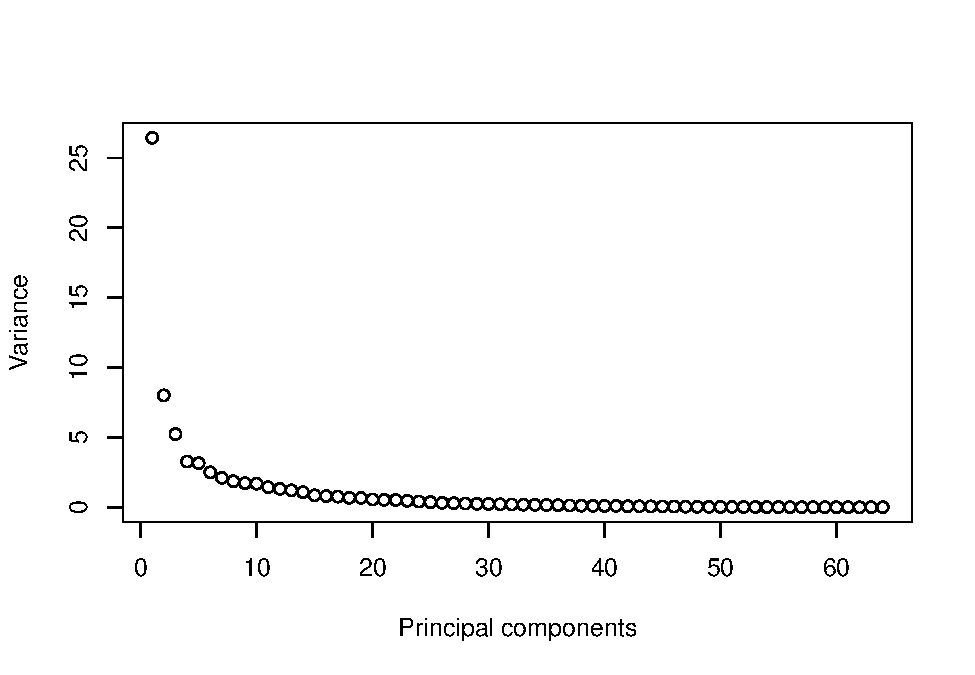
\includegraphics{Supplementary_materials_files/figure-latex/unnamed-chunk-5-1} 

}

\caption{Variance of each principal compnent. Data was fed into the discriminat model to find features separating both species.}\label{fig:unnamed-chunk-5}
\end{figure}

\begin{figure}

{\centering 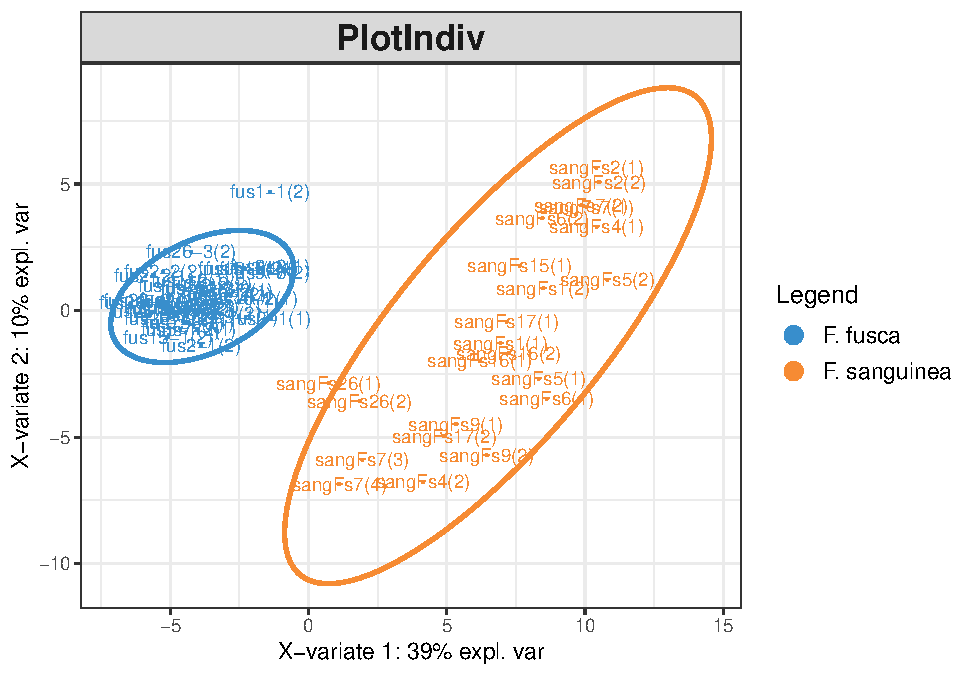
\includegraphics{Supplementary_materials_files/figure-latex/unnamed-chunk-9-1} 

}

\caption{Distribution of the samples projected onto two first latent components before optimizing the number of model paramaters.}\label{fig:unnamed-chunk-9}
\end{figure}

\begin{figure}

{\centering 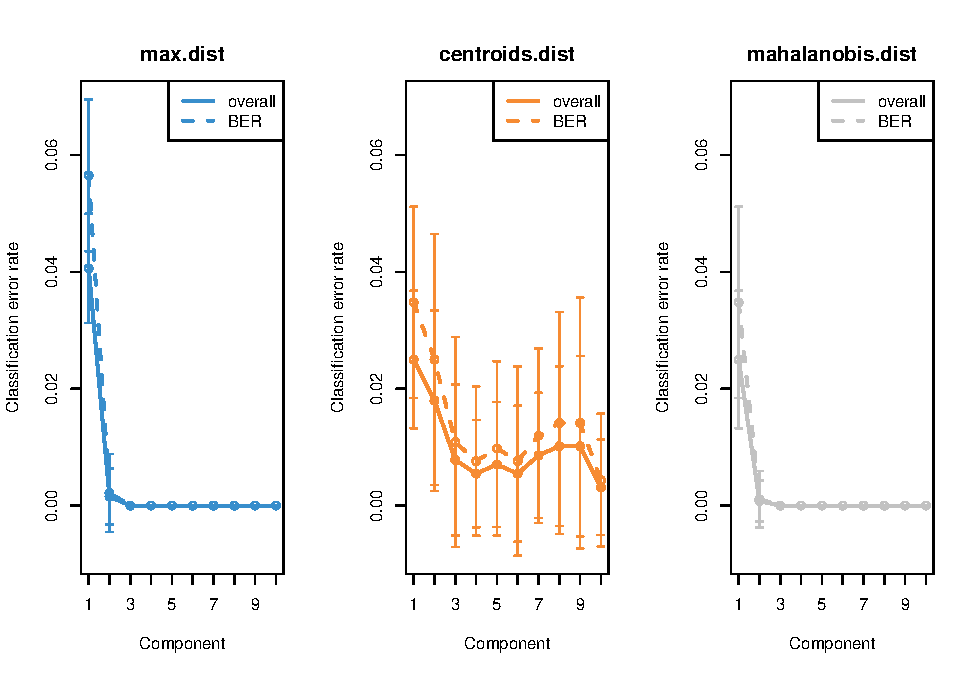
\includegraphics{Supplementary_materials_files/figure-latex/unnamed-chunk-11-1} 

}

\caption{Results of the performance test of the discriminant model with different number of the latent components. For details see the documunetation of R mixOmics package.}\label{fig:unnamed-chunk-11}
\end{figure}

\begin{figure}

{\centering 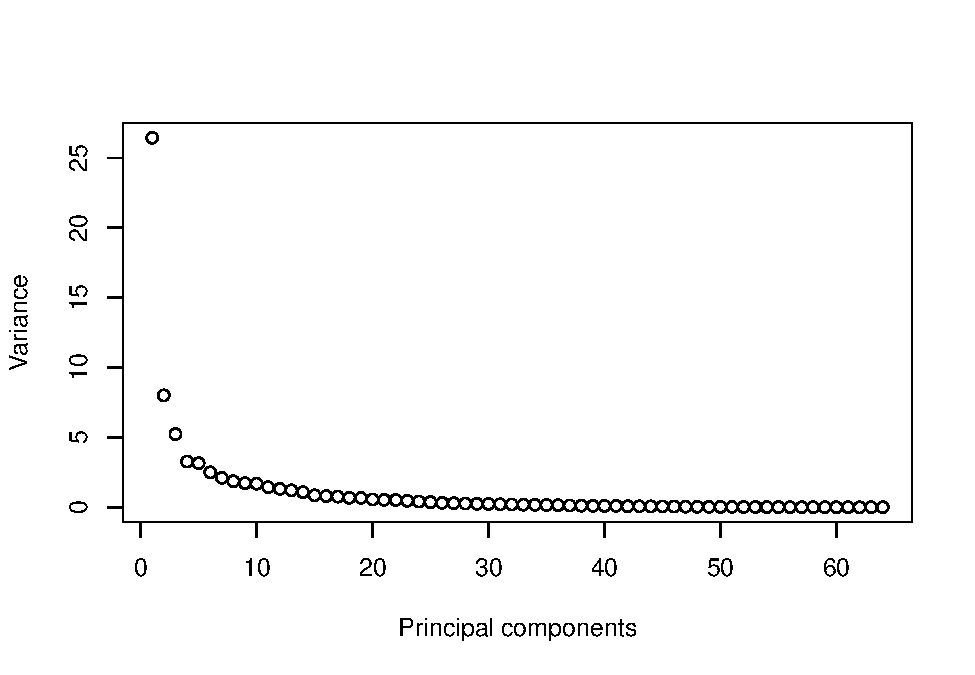
\includegraphics{Supplementary_materials_files/figure-latex/unnamed-chunk-13-1} 

}

\caption{Projection of the samples in onto two first discriminant analysis components after model tuning.}\label{fig:unnamed-chunk-13}
\end{figure}

\begin{longtable}[t]{rlrll}
\caption{\label{tab:unnamed-chunk-15}List of the peaks with the species identity score indicating their importance as a marker of \textit{F. fusca} or \textit{F. sanguinea} samples.}\\
\toprule
Peak ID & Compound & Marker score & fusca marker & sanguinea marker\\
\midrule
\endfirsthead
\caption[]{\label{tab:unnamed-chunk-15}List of the peaks with the species identity score indicating their importance as a marker of \textit{F. fusca} or \textit{F. sanguinea} samples. \textit{(continued)}}\\
\toprule
Peak ID & Compound & Marker score & fusca marker & sanguinea marker\\
\midrule
\endhead

\endfoot
\bottomrule
\endlastfoot
15 & 4-MeC24 & -0.0249041 & TRUE & FALSE\\
60 & 13,17-diMeC29 & -0.0225439 & TRUE & FALSE\\
14 & 6-MeC24 & -0.0183227 & TRUE & FALSE\\
10 & 3-MeC23 & -0.0179422 & TRUE & FALSE\\
19 & 4,12-diMeC24 & -0.0178830 & TRUE & FALSE\\
\addlinespace
12 & 3,13-; 3,11-; 3,9-; 3,7-diMeC23 & -0.0178489 & TRUE & FALSE\\
6 & 11-Me-C23 + 9-Me-C23 & -0.0174140 & TRUE & FALSE\\
7 & 7-Me-C23 & -0.0172762 & TRUE & FALSE\\
33 & 6-MeC26 & -0.0162962 & TRUE & FALSE\\
37 & 7,x-; 5,x-; 10,14-diMeC26 & -0.0161379 & TRUE & FALSE\\
\addlinespace
31 & 3,13-diMeC25 & -0.0159869 & TRUE & FALSE\\
32 & 14-; 10-MeC26 + 3,7,11-triMeC25 & -0.0156195 & TRUE & FALSE\\
13 & 12-; 11-; 10-; 9-; 8-MeC24 & -0.0155301 & TRUE & FALSE\\
49 & 7,11-diMeC27 & -0.0148635 & TRUE & FALSE\\
40 & 4,12-diMeC26 & -0.0138695 & TRUE & FALSE\\
\addlinespace
69 & C31 & -0.0134870 & FALSE & FALSE\\
22 & 13-; 11-; 9-MeC25 & -0.0131439 & FALSE & FALSE\\
21 & 4,12,16-triMeC24 & -0.0131399 & FALSE & FALSE\\
11 & C24 & -0.0125738 & FALSE & FALSE\\
44 & 7-MeC27 & -0.0124500 & FALSE & FALSE\\
\addlinespace
5 & C23 & -0.0118715 & FALSE & FALSE\\
8 & 5-Me C23 & -0.0117793 & FALSE & FALSE\\
27 & 7,11-diMeC25 + 3-MeC25 & -0.0116477 & FALSE & FALSE\\
3 & C23-ene & -0.0111505 & FALSE & FALSE\\
42 & 4,8,14-MeC26 & -0.0097947 & FALSE & FALSE\\
\addlinespace
57 & 4,8,12-triMeC28 & -0.0089917 & FALSE & FALSE\\
55 & C29ene & -0.0089661 & FALSE & FALSE\\
26 & 11,15-; 9,13-diMeC25 & -0.0080687 & FALSE & FALSE\\
65 & 3,7-; 3,9-; 3,11-diMeC29 & -0.0076104 & FALSE & FALSE\\
34 & 5-MeC26 & -0.0066531 & FALSE & FALSE\\
\addlinespace
16 & 10,14-diMeC24 & -0.0061152 & FALSE & FALSE\\
63 & C30ene & -0.0054783 & FALSE & FALSE\\
24 & 7-MeC25 & -0.0033031 & FALSE & FALSE\\
53 & 14-; 12-; 10-MeC28 & -0.0030474 & FALSE & FALSE\\
23 & 9-MeC25 & -0.0020305 & FALSE & FALSE\\
\addlinespace
47 & 9,17-; 9,15-diMeC27 & -0.0004269 & FALSE & FALSE\\
77 & C33ene & 0.0007464 & FALSE & FALSE\\
56 & C29 & 0.0014108 & FALSE & FALSE\\
51 & C28 + 3,15-diMeC27 & 0.0015377 & FALSE & FALSE\\
20 & C25 & 0.0019539 & FALSE & FALSE\\
\addlinespace
58 & 15-; 13-; 11-; 9-; 7-MeC29 & 0.0027182 & FALSE & FALSE\\
28 & 5,13-diMeC25 & 0.0027199 & FALSE & FALSE\\
9 & 9,13-diMeC23 & 0.0034733 & FALSE & FALSE\\
43 & 13-MeC27 & 0.0035200 & FALSE & FALSE\\
59 & 11,17-diMeC29 & 0.0049671 & FALSE & FALSE\\
\addlinespace
66 & 14-; 13-; 12-; 11-MeC30 & 0.0050449 & FALSE & FALSE\\
48 & 9,13-diMeC27 & 0.0051735 & FALSE & FALSE\\
4 & C23-ene & 0.0062418 & FALSE & FALSE\\
52 & 3,9-; 3,7-diMeC27 & 0.0074584 & FALSE & FALSE\\
18 & C25-ene & 0.0075198 & FALSE & FALSE\\
\addlinespace
36 & 10,16-; 10,14-diMeC26 & 0.0086021 & FALSE & FALSE\\
72 & 13,19-;13,17-diMeC31 & 0.0093329 & FALSE & FALSE\\
80 & 11,21-; 11,19-diMeC33 & 0.0098888 & FALSE & FALSE\\
54 & 8,12,16-triMeC28 & 0.0103398 & FALSE & FALSE\\
75 & x-Me\_C32 & 0.0113011 & FALSE & FALSE\\
\addlinespace
62 & 5,9-; 5,11-; 5,13-diMeC29 & 0.0116546 & FALSE & FALSE\\
35 & 4-MeC26 & 0.0120883 & FALSE & TRUE\\
30 & C26 & 0.0127907 & FALSE & TRUE\\
79 & x-Me\_C32 & 0.0132805 & FALSE & TRUE\\
17 & C25-ene & 0.0148301 & FALSE & TRUE\\
\addlinespace
74 & (di)MeC31, mix & 0.0149467 & FALSE & TRUE\\
45 & 5-MeC27 & 0.0150032 & FALSE & TRUE\\
46 & 11,15-diMeC27 & 0.0151218 & FALSE & TRUE\\
76 & 13,17-DiMe\_C32 + x,y-DiMe\_C32 & 0.0154345 & FALSE & TRUE\\
70 & 15-; 13-; 11-; 9-MeC31 & 0.0155745 & FALSE & TRUE\\
\addlinespace
71 & 11,19-; 11,17-; 11,15-diMeC31 & 0.0181955 & FALSE & TRUE\\
38 & C27-ene + 6,12-diMeC26 & 0.0190222 & FALSE & TRUE\\
41 & C27 & 0.0214514 & FALSE & TRUE\\
67 & (di)MeC30 (mix) & 0.0282812 & FALSE & TRUE\\
25 & 5-MeC25 & 0.0297436 & FALSE & TRUE\\
\addlinespace
50 & C28ene & 0.0316220 & FALSE & TRUE\\*
\end{longtable}

\subsection{Species Identity Score}\label{species-identity-score}

Ants in the mixed colonies exchanged their CHC to produce a hybrid chemical identity. We developed a method to assign each sample a value measuring similarity to one or the other species. It is based on a discriminant model that predicts the class of new samples using \texttt{predict} method from \texttt{mixOmics} R package. The input data are processed in the same way as the training set, i.e.~central-log transformation is followed by projection into principal component space. In the latter step, the same rotation matrix and scaling vector is applied as those used for the training set are applied. This is achieved by using \texttt{predict} method on the object of \texttt{prcomp} class.

\subsubsection{\texorpdfstring{Predicted species of different categories of ants as a function of the proportion of \emph{F. sanguinea} ants in a colony}{Predicted species of different categories of ants as a function of the proportion of F. sanguinea ants in a colony}}\label{predicted-species-of-different-categories-of-ants-as-a-function-of-the-proportion-of-f.-sanguinea-ants-in-a-colony}

The Species Identity Score was computed for \emph{F. sanguinea} and \emph{F. fusca} samples from mixed colonies and used as a response variable in linear mixed models. As a fixed effect we used the proportion of \emph{F. sanguinea} workers among all workers in a colony. Colony ID and sampling occasion were incorporated as random effects.

In the following model specifications \((1|\text{random_factor})\) denotes random intercept (separate for each level of the random factor) and \(((1|\text{random_factor_1:random_factor_2}))\) denotes random intercepts generated from the combinations of two factors. \(\beta_{0}\) and \(\epsilon\) denote intercept and error term, respectively. Included are summary reports, results of the Shapiro-Wilk test of nornalizty of conditional residuals, as well as diagnostic plots and tests generated with the use of \texttt{DHARMa} R package\citep{R-DHARMa}. The response variable often needed to be transformed to meet model assumptions. Random terms with no variance have been dropped.

\paragraph{\texorpdfstring{Mature \emph{F. sanguinea}}{Mature F. sanguinea}}\label{mature-f.-sanguinea}

\[
\sqrt{\text{Species_Identity_Score}} = \beta_0 + \text{sanguinea_proportion} + (1|\text{colony_ID:sampling_occasion_ID}) + \epsilon,
\]
where \(\text{Species_Identity_Score}\) denotes the Species Identity Score of the mature \emph{F. sanguinea} workers.

\begin{verbatim}
## Linear mixed model fit by REML. t-tests use Satterthwaite's method ['lmerModLmerTest']
## Formula: I(sqrt(predicted_species)) ~ sang_prop + (1 | colony:census_date)
##    Data: model_input
## 
## REML criterion at convergence: 15.1
## 
## Scaled residuals: 
##      Min       1Q   Median       3Q      Max 
## -1.67059 -0.70651  0.03909  0.45140  2.13865 
## 
## Random effects:
##  Groups             Name        Variance Std.Dev.
##  colony:census_date (Intercept) 0.03547  0.1883  
##  Residual                       0.04090  0.2022  
## Number of obs: 55, groups:  colony:census_date, 38
## 
## Fixed effects:
##             Estimate Std. Error       df t value Pr(>|t|)    
## (Intercept)  0.70476    0.07965 40.25725   8.849 5.49e-11 ***
## sang_prop    1.02077    0.14311 37.99116   7.133 1.63e-08 ***
## ---
## Signif. codes:  0 '***' 0.001 '**' 0.01 '*' 0.05 '.' 0.1 ' ' 1
## 
## Correlation of Fixed Effects:
##           (Intr)
## sang_prop -0.853
\end{verbatim}

\begin{verbatim}
## 
##  Shapiro-Wilk normality test
## 
## data:  residuals(lm_model)
## W = 0.98367, p-value = 0.657
\end{verbatim}

\begin{center}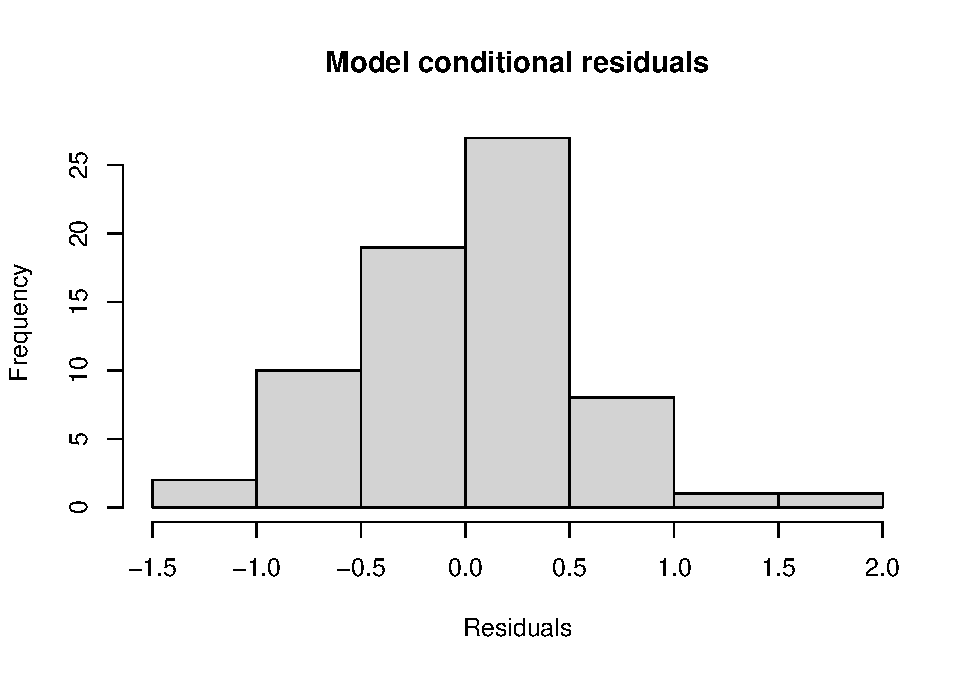
\includegraphics{Supplementary_materials_files/figure-latex/unnamed-chunk-18-1} 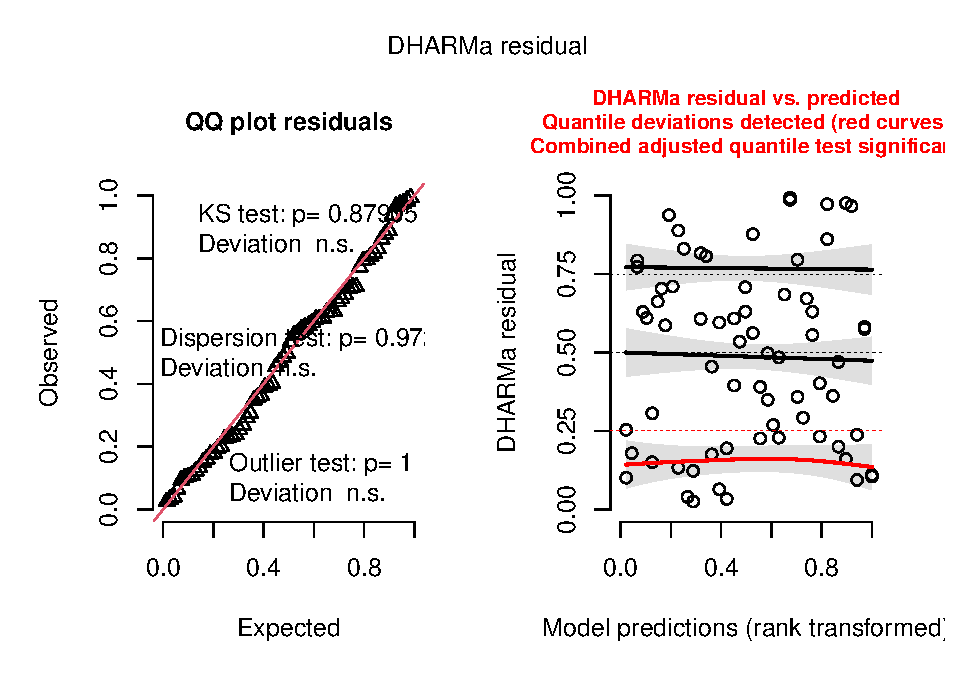
\includegraphics{Supplementary_materials_files/figure-latex/unnamed-chunk-18-2} \end{center}

\paragraph{\texorpdfstring{\emph{F. fusca}}{F. fusca}}\label{f.-fusca}

\[
\text{Species_Identity_Score}= \beta_0 + \text{sanguinea_proportion} + (1|\text{colony})+(1|\text{colony_ID:sampling_occasion_ID}) + \epsilon,
\]
where \(\text{Species_Identity_Score}\) denotes the Species Identity Score of the mature \emph{F. fusca} workers.

\begin{verbatim}
## Linear mixed model fit by REML. t-tests use Satterthwaite's method ['lmerModLmerTest']
## Formula: predicted_species ~ sang_prop + (1 | colony) + (1 | colony:census_date)
##    Data: model_input
## 
## REML criterion at convergence: 230.1
## 
## Scaled residuals: 
##      Min       1Q   Median       3Q      Max 
## -2.84293 -0.49799 -0.00101  0.51466  2.30723 
## 
## Random effects:
##  Groups             Name        Variance Std.Dev.
##  colony:census_date (Intercept) 0.2786   0.5278  
##  colony             (Intercept) 0.1613   0.4016  
##  Residual                       0.7560   0.8695  
## Number of obs: 78, groups:  colony:census_date, 55; colony, 20
## 
## Fixed effects:
##             Estimate Std. Error      df t value Pr(>|t|)    
## (Intercept)  -1.1567     0.2046 41.7318  -5.653 1.28e-06 ***
## sang_prop     3.4941     0.4413 37.9240   7.917 1.48e-09 ***
## ---
## Signif. codes:  0 '***' 0.001 '**' 0.01 '*' 0.05 '.' 0.1 ' ' 1
## 
## Correlation of Fixed Effects:
##           (Intr)
## sang_prop -0.648
\end{verbatim}

\begin{verbatim}
## 
##  Shapiro-Wilk normality test
## 
## data:  residuals(lm_model)
## W = 0.98191, p-value = 0.3341
\end{verbatim}

\begin{center}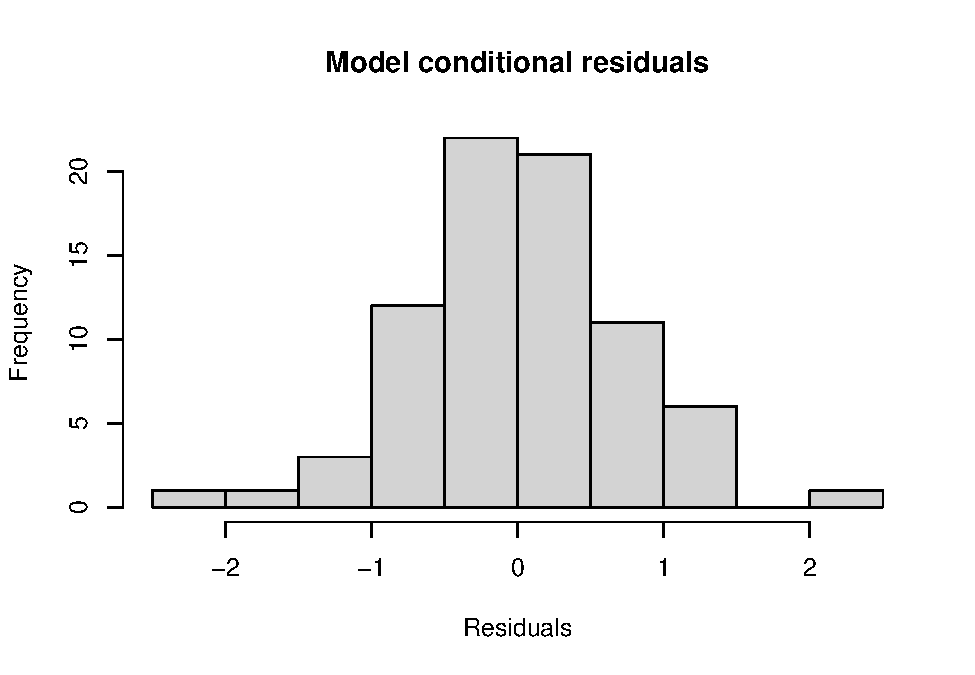
\includegraphics{Supplementary_materials_files/figure-latex/unnamed-chunk-19-1} 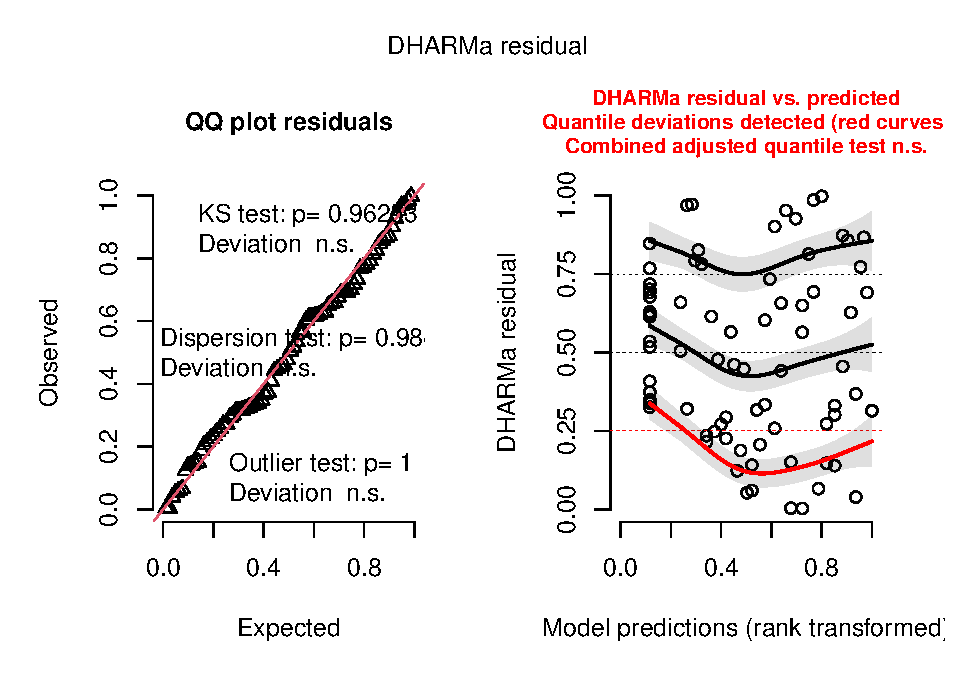
\includegraphics{Supplementary_materials_files/figure-latex/unnamed-chunk-19-2} \end{center}

\paragraph{\texorpdfstring{Callow \emph{F. sanguinea}}{Callow F. sanguinea}}\label{callow-f.-sanguinea}

\[
\text{Species_Identity_Score}= \beta_0 + \text{sanguinea_proportion} + (1|\text{colony}) + \epsilon,
\]
where \(\text{Species_Identity_Score}\) denotes the Species Identity Score of the callow \emph{F. sanguinea} workers.

\begin{verbatim}
## Linear mixed model fit by REML. t-tests use Satterthwaite's method ['lmerModLmerTest']
## Formula: predicted_species ~ sang_prop + (1 | colony)
##    Data: model_input
## 
## REML criterion at convergence: 76.1
## 
## Scaled residuals: 
##      Min       1Q   Median       3Q      Max 
## -2.02656 -0.63913 -0.06358  0.80146  1.76498 
## 
## Random effects:
##  Groups   Name        Variance Std.Dev.
##  colony   (Intercept) 0.08451  0.2907  
##  Residual             0.56151  0.7493  
## Number of obs: 32, groups:  colony, 16
## 
## Fixed effects:
##             Estimate Std. Error      df t value Pr(>|t|)    
## (Intercept)  -0.5935     0.2554 28.9222  -2.324   0.0274 *  
## sang_prop     2.4749     0.4663 28.3415   5.308 1.15e-05 ***
## ---
## Signif. codes:  0 '***' 0.001 '**' 0.01 '*' 0.05 '.' 0.1 ' ' 1
## 
## Correlation of Fixed Effects:
##           (Intr)
## sang_prop -0.798
\end{verbatim}

\begin{verbatim}
## 
##  Shapiro-Wilk normality test
## 
## data:  residuals(lm_model)
## W = 0.97007, p-value = 0.5014
\end{verbatim}

\begin{center}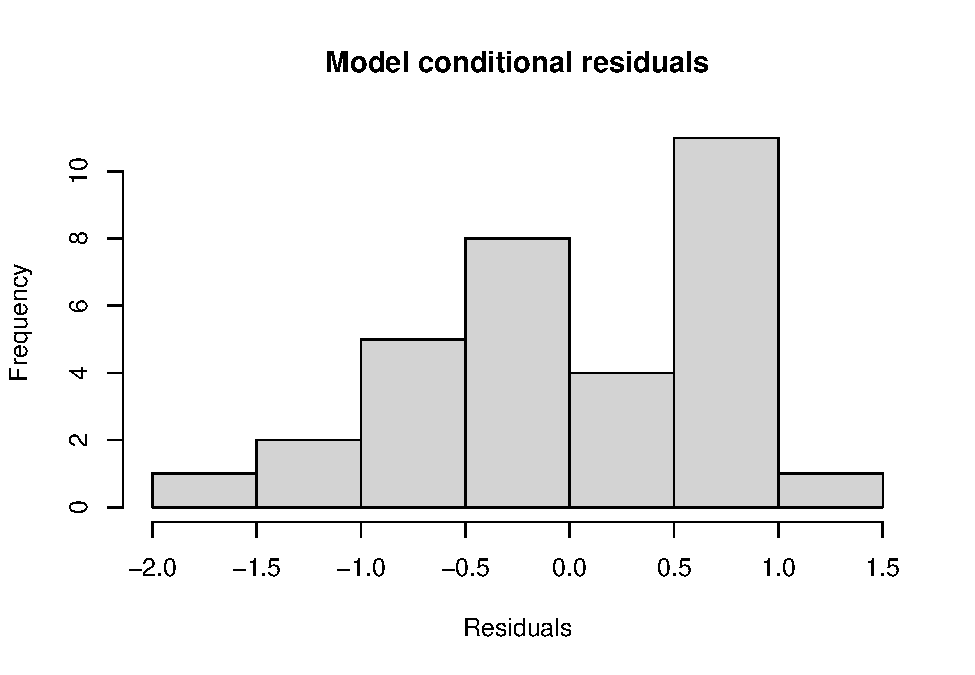
\includegraphics{Supplementary_materials_files/figure-latex/unnamed-chunk-20-1} 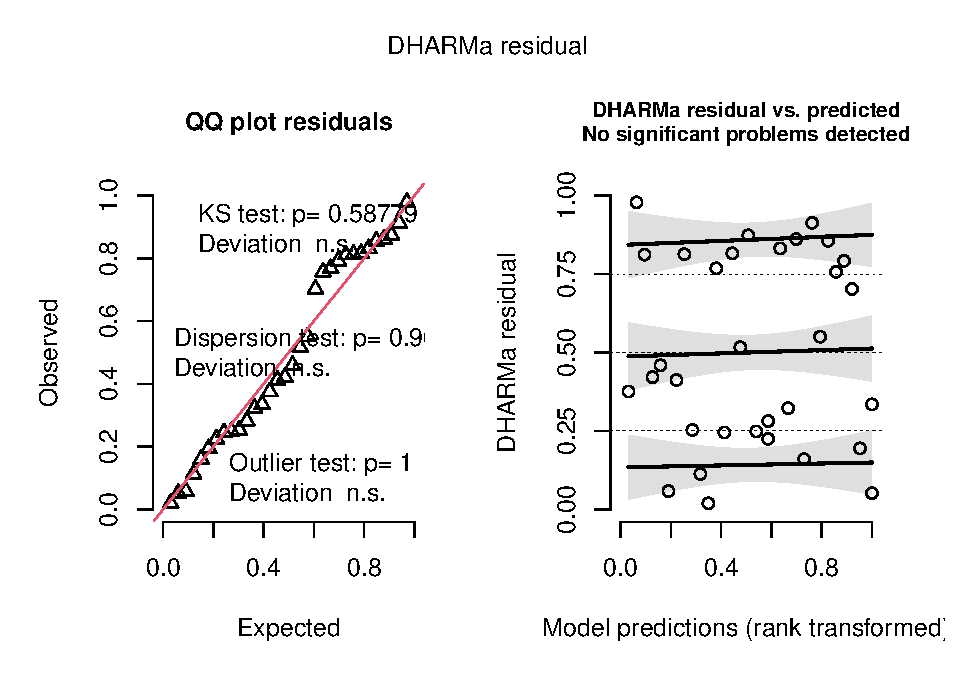
\includegraphics{Supplementary_materials_files/figure-latex/unnamed-chunk-20-2} \end{center}

\subsubsection{\texorpdfstring{Difference in Species Identity Score between mature \emph{F. sanguinea} ants and \emph{F. fusca} slaves}{Difference in Species Identity Score between mature F. sanguinea ants and F. fusca slaves}}\label{difference-in-species-identity-score-between-mature-f.-sanguinea-ants-and-f.-fusca-slaves}

Since the linear model does not meet one of diagnostics criteria, a Wilcoxon paired test was applied.

\begin{verbatim}
## 
##  Wilcoxon signed rank test with continuity correction
## 
## data:  model_input$predicted_species and model_input$slave_species_index
## V = 1843, p-value = 4.856e-07
## alternative hypothesis: true location shift is not equal to 0
\end{verbatim}

\begin{center}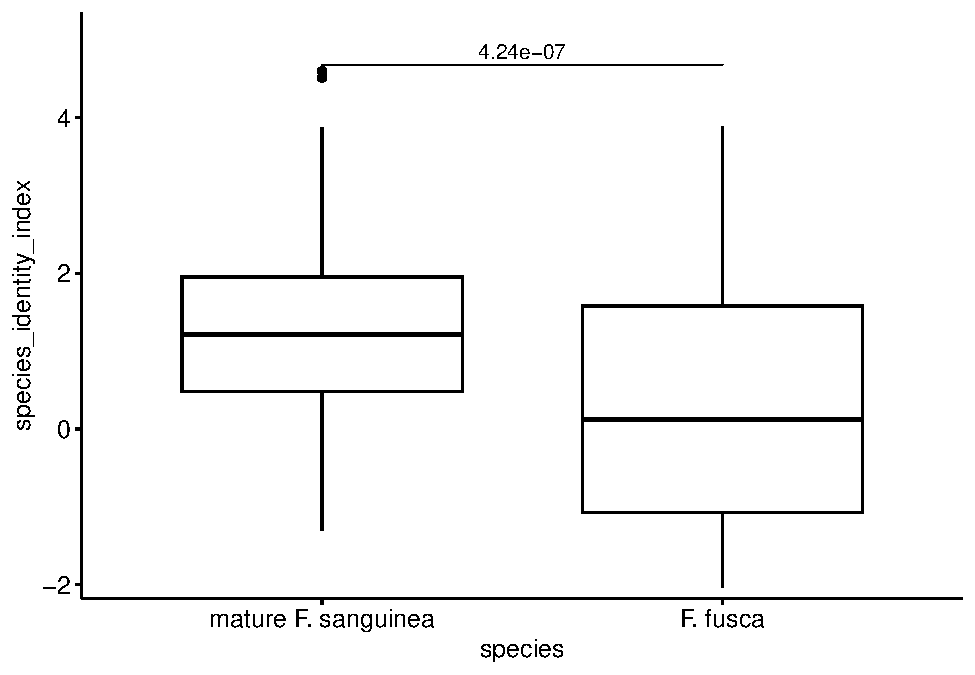
\includegraphics{Supplementary_materials_files/figure-latex/unnamed-chunk-21-1} \end{center}

\subsubsection{\texorpdfstring{Difference in Species Identity Score between callow \emph{F. sanguinea} ants and \emph{F. fusca} slaves}{Difference in Species Identity Score between callow F. sanguinea ants and F. fusca slaves}}\label{difference-in-species-identity-score-between-callow-f.-sanguinea-ants-and-f.-fusca-slaves}

\[
\text{SIS_diff}= \beta_0 + \text{sanguinea_proportion} + (1|\text{colony}) + \epsilon,
\]
where \(\text{SIS_diff}\) denotes the difference in Species Identity Score between the mature \emph{F. sanguinea} and \emph{F. fusca} sampled at the same time and from the same colony. Replicated samples were averaged before the calculations.

Since the linear model does not meet one of diagnostics criterion we will apply Wilcoxon paired test.

\begin{verbatim}
## 
## Call:
## lm(formula = index_diff ~ sang_prop, data = model_input)
## 
## Residuals:
##     Min      1Q  Median      3Q     Max 
## -2.4185 -0.6058 -0.1187  0.7012  1.7033 
## 
## Coefficients:
##             Estimate Std. Error t value Pr(>|t|)
## (Intercept)   0.4099     0.3321   1.234    0.227
## sang_prop    -0.6889     0.6849  -1.006    0.323
## 
## Residual standard error: 1.013 on 28 degrees of freedom
##   (2 observations deleted due to missingness)
## Multiple R-squared:  0.03488,    Adjusted R-squared:  0.0004127 
## F-statistic: 1.012 on 1 and 28 DF,  p-value: 0.323
\end{verbatim}

\begin{verbatim}
## 
##  Shapiro-Wilk normality test
## 
## data:  residuals(lm_model)
## W = 0.97214, p-value = 0.5992
\end{verbatim}

\begin{center}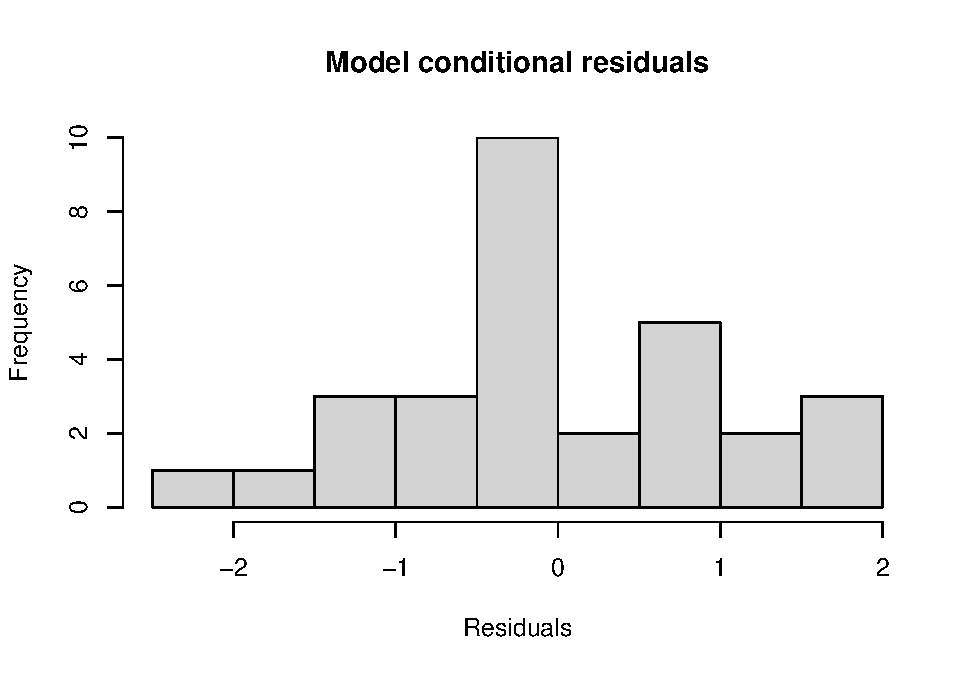
\includegraphics{Supplementary_materials_files/figure-latex/unnamed-chunk-22-1} \end{center}

\subsubsection{\texorpdfstring{Difference in Species Identity Score between callow and mature \emph{F. sanguinea} ants.}{Difference in Species Identity Score between callow and mature F. sanguinea ants.}}\label{difference-in-species-identity-score-between-callow-and-mature-f.-sanguinea-ants.}

\begin{verbatim}
## 
## Call:
## lm(formula = index_diff ~ sang_prop, data = model_input)
## 
## Residuals:
##      Min       1Q   Median       3Q      Max 
## -2.31963 -0.51182 -0.08442  0.67933  1.85442 
## 
## Coefficients:
##             Estimate Std. Error t value Pr(>|t|)  
## (Intercept)  -0.7008     0.3147  -2.227   0.0342 *
## sang_prop    -0.1707     0.5758  -0.297   0.7690  
## ---
## Signif. codes:  0 '***' 0.001 '**' 0.01 '*' 0.05 '.' 0.1 ' ' 1
## 
## Residual standard error: 0.9399 on 28 degrees of freedom
##   (2 observations deleted due to missingness)
## Multiple R-squared:  0.003131,   Adjusted R-squared:  -0.03247 
## F-statistic: 0.08793 on 1 and 28 DF,  p-value: 0.769
\end{verbatim}

\begin{verbatim}
## 
##  Shapiro-Wilk normality test
## 
## data:  residuals(lm_model)
## W = 0.98622, p-value = 0.9561
\end{verbatim}

\begin{center}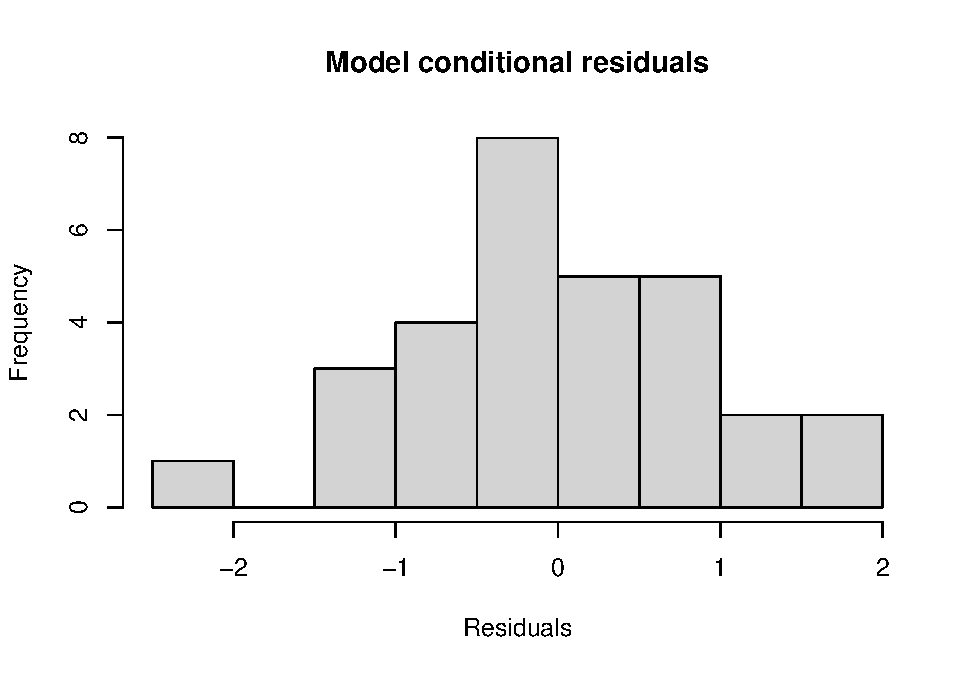
\includegraphics{Supplementary_materials_files/figure-latex/unnamed-chunk-23-1} \end{center}

\section{\texorpdfstring{Finding peaks differentiating callow and mature \emph{F. sanguinea} workers}{Finding peaks differentiating callow and mature F. sanguinea workers}}\label{finding-peaks-differentiating-callow-and-mature-f.-sanguinea-workers}

The procedure identifying species markers was also applied to determine peaks characteristic of \emph{F. sanguinea} callow ants. In discriminant analysis, samples were classified into one of the three groups: callow \emph{F. sanguinea}, adult \emph{F. sanguinea}, or adult \emph{F. fusca}.

\begin{figure}

{\centering 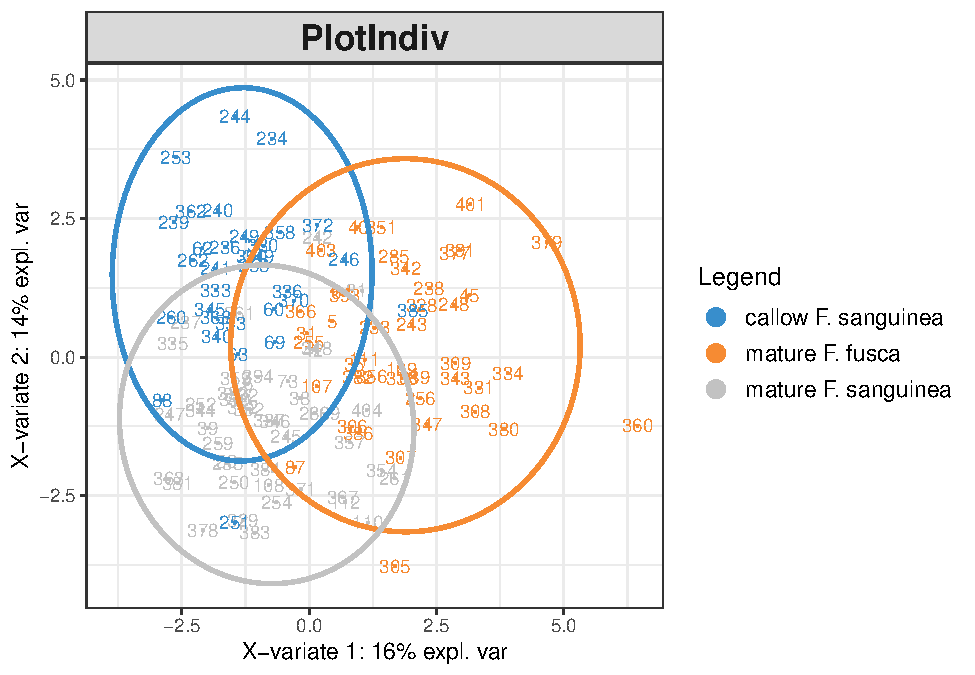
\includegraphics{Supplementary_materials_files/figure-latex/unnamed-chunk-26-1} 

}

\caption{Distribution of the samples projected onto two first latent components before optimizing the number of model paramaters.}\label{fig:unnamed-chunk-26}
\end{figure}

\begin{figure}

{\centering 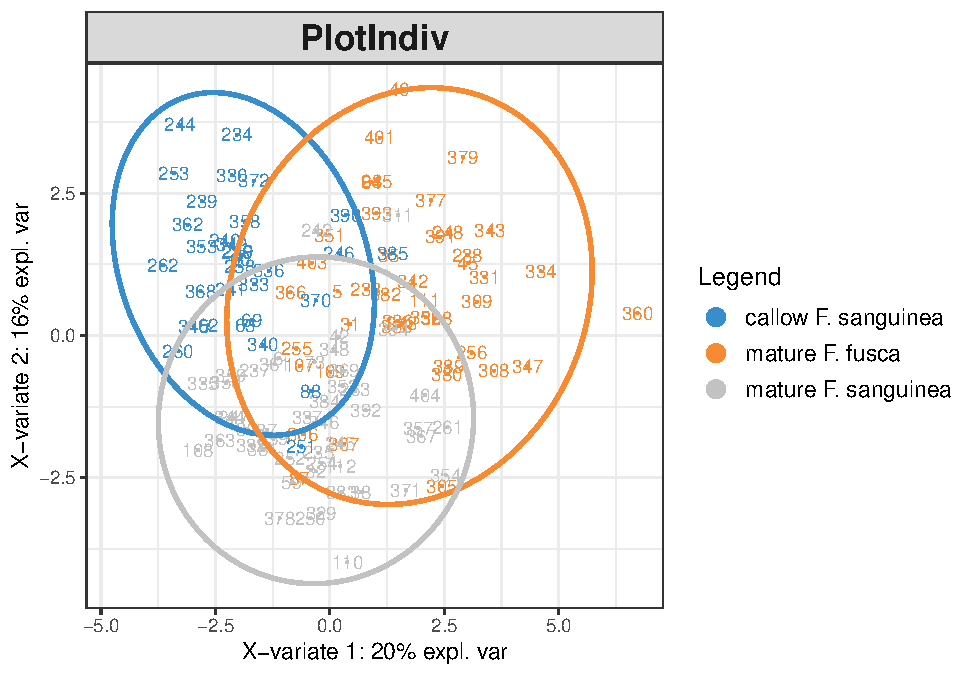
\includegraphics{Supplementary_materials_files/figure-latex/unnamed-chunk-28-1} 

}

\caption{Projection of the samples in onto two first discriminant analysis components after model tuning.}\label{fig:unnamed-chunk-28}
\end{figure}

\begin{longtable}[t]{rlrlrl}
\caption{\label{tab:unnamed-chunk-30}List of the peaks with the score indicating their importance as a marker of mature \textit{F. fusca}, mature \textit{F. sanguinea}, or callow \textit{F. sanguinea} samples.}\\
\toprule
Peak ID & Compound & Callow score & Callow marker & Mature score & Mature marker\\
\midrule
\endfirsthead
\caption[]{\label{tab:unnamed-chunk-30}List of the peaks with the score indicating their importance as a marker of mature \textit{F. fusca}, mature \textit{F. sanguinea}, or callow \textit{F. sanguinea} samples. \textit{(continued)}}\\
\toprule
Peak ID & Compound & Callow score & Callow marker & Mature score & Mature marker\\
\midrule
\endhead

\endfoot
\bottomrule
\endlastfoot
68 & C31ene; 3-MeC30 & 0.1130847 & TRUE & -0.0902940 & FALSE\\
77 & C33ene & 0.0674065 & TRUE & -0.0358531 & FALSE\\
43 & 13-MeC27 & 0.0660307 & TRUE & -0.0176578 & FALSE\\
32 & 14-; 10-MeC26 + 3,7,11-triMeC25 & 0.0566271 & TRUE & -0.0470084 & FALSE\\
53 & 14-; 12-; 10-MeC28 & 0.0548579 & TRUE & -0.0275054 & FALSE\\
\addlinespace
58 & 15-; 13-; 11-; 9-; 7-MeC29 & 0.0489691 & TRUE & 0.0004851 & FALSE\\
22 & 13-; 11-; 9-MeC25 & 0.0448772 & TRUE & -0.0571426 & FALSE\\
13 & 12-; 11-; 10-; 9-; 8-MeC24 & 0.0364630 & TRUE & -0.0599463 & FALSE\\
28 & 5,13-diMeC25 & 0.0280841 & TRUE & -0.0276607 & FALSE\\
19 & 4,12-diMeC24 & 0.0279189 & TRUE & -0.0536605 & FALSE\\
\addlinespace
31 & 3,13-diMeC25 & 0.0277922 & TRUE & -0.0257284 & FALSE\\
66 & 14-; 13-; 12-; 11-MeC30 & 0.0263989 & TRUE & -0.0202339 & FALSE\\
38 & C27-ene + 6,12-diMeC26 & 0.0261492 & FALSE & 0.0197898 & FALSE\\
24 & 7-MeC25 & 0.0255483 & FALSE & -0.0057152 & FALSE\\
10 & 3-MeC23 & 0.0234896 & FALSE & -0.0308856 & FALSE\\
\addlinespace
64 & C30 & 0.0187834 & FALSE & -0.0368979 & FALSE\\
5 & C23 & 0.0179810 & FALSE & -0.0306055 & FALSE\\
45 & 5-MeC27 & 0.0155024 & FALSE & 0.0260230 & FALSE\\
52 & 3,9-; 3,7-diMeC27 & 0.0102577 & FALSE & -0.0312129 & FALSE\\
71 & 11,19-; 11,17-; 11,15-diMeC31 & 0.0093526 & FALSE & 0.0435967 & TRUE\\
\addlinespace
6 & 11-Me-C23 + 9-Me-C23 & 0.0092063 & FALSE & -0.0222486 & FALSE\\
12 & 3,13-; 3,11-; 3,9-; 3,7-diMeC23 & 0.0089605 & FALSE & -0.0218476 & FALSE\\
70 & 15-; 13-; 11-; 9-MeC31 & 0.0086096 & FALSE & 0.0291918 & FALSE\\
78 & x-Me-C32 & 0.0059607 & FALSE & -0.0253181 & FALSE\\
79 & x-Me\_C32 & 0.0046869 & FALSE & 0.0085653 & FALSE\\
\addlinespace
50 & C28ene & 0.0035810 & FALSE & 0.0362238 & TRUE\\
49 & 7,11-diMeC27 & 0.0035568 & FALSE & -0.0346106 & FALSE\\
56 & C29 & 0.0014290 & FALSE & -0.0378337 & FALSE\\
60 & 13,17-diMeC29 & 0.0009481 & FALSE & 0.0151416 & FALSE\\
26 & 11,15-; 9,13-diMeC25 & -0.0038959 & FALSE & -0.0078690 & FALSE\\
\addlinespace
47 & 9,17-; 9,15-diMeC27 & -0.0041782 & FALSE & -0.0065953 & FALSE\\
27 & 7,11-diMeC25 + 3-MeC25 & -0.0043027 & FALSE & 0.0375409 & TRUE\\
23 & 9-MeC25 & -0.0046829 & FALSE & 0.0219543 & FALSE\\
36 & 10,16-; 10,14-diMeC26 & -0.0065927 & FALSE & 0.0077764 & FALSE\\
75 & x-Me\_C32 & -0.0078838 & FALSE & 0.0041896 & FALSE\\
\addlinespace
30 & C26 & -0.0083596 & FALSE & -0.0016878 & FALSE\\
37 & 7,x-; 5,x-; 10,14-diMeC26 & -0.0117943 & FALSE & -0.0474630 & FALSE\\
54 & 8,12,16-triMeC28 & -0.0124810 & FALSE & 0.0268892 & FALSE\\
3 & C23-ene & -0.0161920 & FALSE & -0.0380185 & FALSE\\
11 & C24 & -0.0176539 & FALSE & -0.0210220 & FALSE\\
\addlinespace
46 & 11,15-diMeC27 & -0.0244479 & FALSE & 0.0612482 & TRUE\\
25 & 5-MeC25 & -0.0245862 & FALSE & 0.0606407 & TRUE\\
51 & C28 + 3,15-diMeC27 & -0.0247170 & FALSE & 0.0199851 & FALSE\\
20 & C25 & -0.0251803 & FALSE & -0.0101043 & FALSE\\
61 & 7,11-; 7,13-; 7,15-diMeC29 & -0.0255085 & FALSE & 0.0354476 & TRUE\\
\addlinespace
48 & 9,13-diMeC27 & -0.0262900 & FALSE & 0.0347272 & TRUE\\
7 & 7-Me-C23 & -0.0265325 & FALSE & -0.0002857 & FALSE\\
17 & C25-ene & -0.0284637 & FALSE & 0.0614603 & TRUE\\
67 & (di)MeC30 (mix) & -0.0289253 & FALSE & 0.0555200 & TRUE\\
59 & 11,17-diMeC29 & -0.0321720 & FALSE & 0.0333428 & FALSE\\
\addlinespace
44 & 7-MeC27 & -0.0322311 & FALSE & -0.0112348 & FALSE\\
72 & 13,19-;13,17-diMeC31 & -0.0362628 & FALSE & 0.0083934 & FALSE\\
80 & 11,21-; 11,19-diMeC33 & -0.0391225 & FALSE & 0.0484717 & TRUE\\
69 & C31 & -0.0458503 & FALSE & -0.0094236 & FALSE\\
76 & 13,17-DiMe\_C32 + x,y-DiMe\_C32 & -0.0677400 & FALSE & 0.0968633 & TRUE\\
\addlinespace
41 & C27 & -0.0689956 & FALSE & 0.0381717 & TRUE\\*
\end{longtable}

\subsection{Verifying the performace of the discrimination model}\label{verifying-the-performace-of-the-discrimination-model}

The performance of the discriminant model was evaluated by examining the accuracy of its predictions in a cross-validation test, measured as the area under the receiver operating characteristic curve (AUROC). This procedure was repeated \(10^3\) times to account for variance resulting from the random splitting of samples into training and validation sets. In a parallel analysis, the model was trained on data with permuted age status of \emph{F. sanguinea} to assess whether the true assignment of samples influenced model performance. Results from both training approaches were paired, and the difference in AUROC was calculated each for pair. The empirical p-value was defined as the proportion of models in which the AUROC after permutation was equal to or greater than the AUROC based on the original data.

The p-value is calculated as proportion of differences with value equal to or less than zero.

\begin{figure}

{\centering 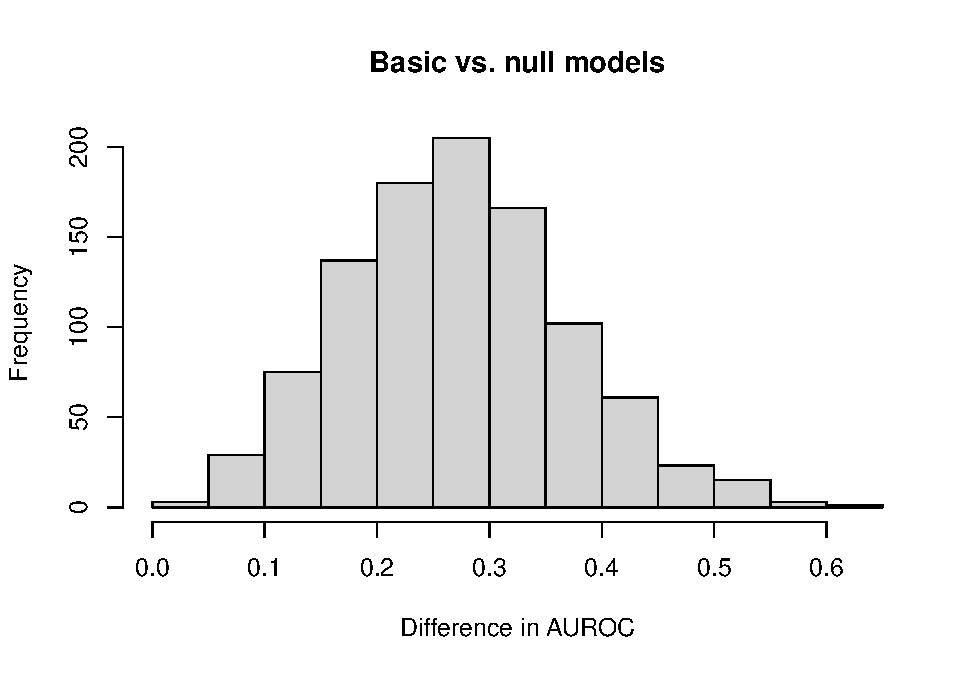
\includegraphics{Supplementary_materials_files/figure-latex/unnamed-chunk-34-1} 

}

\caption{Distribution of the differences in the performance of the discriminant models trained on true and permuted data. Age status of \textit{F. sanguinea} ants were shuffled in the null variant.}\label{fig:unnamed-chunk-34}
\end{figure}

All differences are positive, so the \emph{p}-value is less than 0.001 since the null distribution consists of 1000 values.

\section{Changes of CHC amount over time}\label{changes-of-chc-amount-over-time}

This section contains a series of linear (mixed) models fitted to examine how the proportion of \emph{F. sanguinea} workers in a colony is associated with the amount of CHC, analyzed as a whole or in subsets. Included are summary reports, results of the Shapiro-Wilk test of normality of conditional residuals, as well as diagnostic plots and tests generated with the use of \texttt{DHARMa} R package\citep{R-DHARMa}. The response variable often needed to be transformed to meet model assumptions. Random terms with no variance have been dropped.

In model specification \((1|\text{random_factor})\) denotes random intercept (separate for each level of the random factor) and \(((1|\text{random_factor_1:random_factor_2}))\) denotes random intercepts generated from the combinations of two factors. \(\beta_{0}\) and \(\epsilon\) denote intercept and error term, respectively.

\subsection{Colony growth and body size}\label{colony-growth-and-body-size}

In the analyses below, the normalized CHC amounts were used as a response variable. Since the body shape in both species deviates from isometric growth pattern (see Section @ref(surface\_area)), the CHC amount normalization by the square of head width might bias the calculations. To account for that we first examine the relationship between body size (head width) and proportion of \emph{F. sanguinea} worker in a colony and next we incorporate the square of head width as an explanatory variable to the linear model.

\[
\text{head_width} =  \beta_0 + \text{sanguinea_proportion} + (1|\text{colony_ID}) + \epsilon,
\]

\begin{verbatim}
## Linear mixed model fit by REML. t-tests use Satterthwaite's method ['lmerModLmerTest']
## Formula: head_width ~ sang_prop + (1 | colony)
##    Data: model_input
## 
## REML criterion at convergence: 808
## 
## Scaled residuals: 
##      Min       1Q   Median       3Q      Max 
## -2.10138 -0.61076  0.06058  0.43106  2.28980 
## 
## Random effects:
##  Groups   Name        Variance Std.Dev.
##  colony   (Intercept) 3155     56.17   
##  Residual             9110     95.45   
## Number of obs: 68, groups:  colony, 16
## 
## Fixed effects:
##             Estimate Std. Error      df t value Pr(>|t|)    
## (Intercept)  1218.06      26.41   38.93  46.121  < 2e-16 ***
## sang_prop     125.14      43.44   62.10   2.881  0.00544 ** 
## ---
## Signif. codes:  0 '***' 0.001 '**' 0.01 '*' 0.05 '.' 0.1 ' ' 1
## 
## Correlation of Fixed Effects:
##           (Intr)
## sang_prop -0.715
\end{verbatim}

\begin{verbatim}
## 
##  Shapiro-Wilk normality test
## 
## data:  residuals(lm_model)
## W = 0.9861, p-value = 0.6514
\end{verbatim}

\begin{center}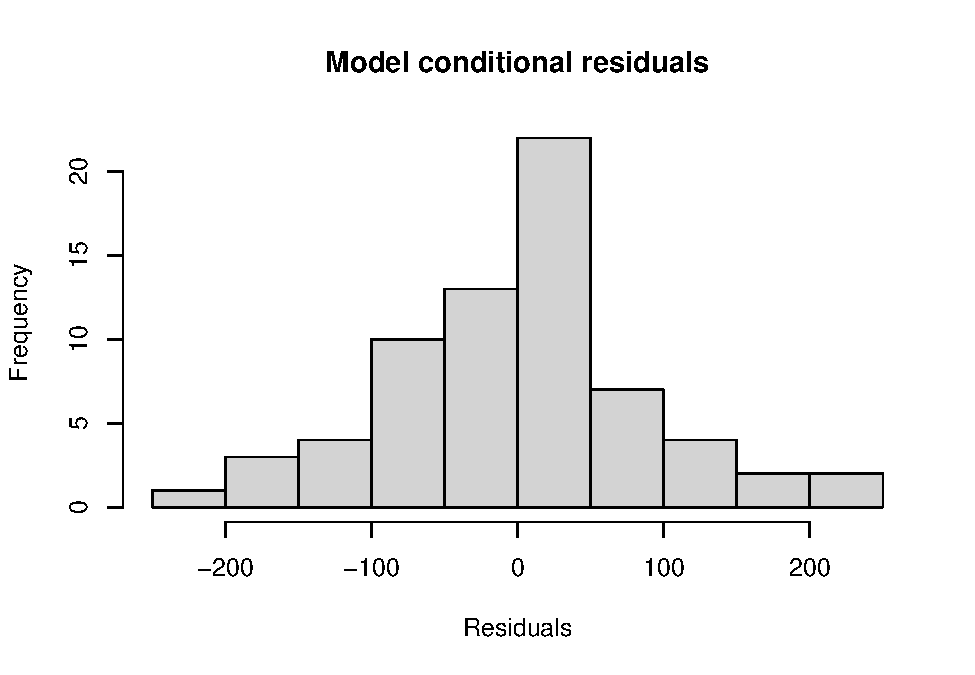
\includegraphics{Supplementary_materials_files/figure-latex/unnamed-chunk-36-1} 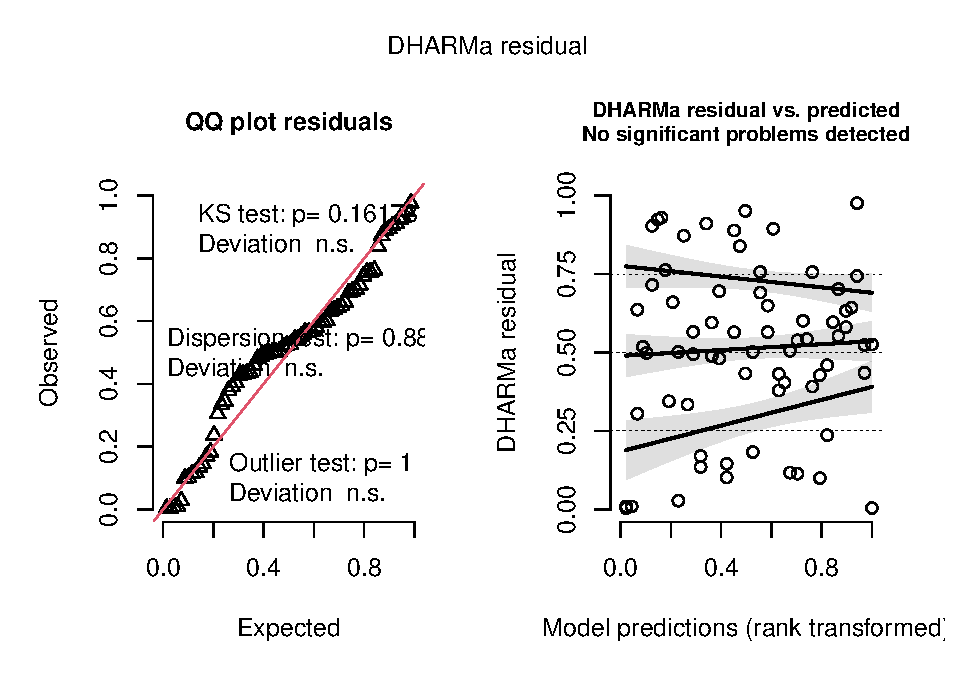
\includegraphics{Supplementary_materials_files/figure-latex/unnamed-chunk-36-2} \end{center}

\subsection{Change in the total CHCs mass}\label{change-in-the-total-chcs-mass}

In this series of models the total CHC mass (normalized by assuming head width of 1.3 mm) was regressed on the proportion of \emph{Formica sanguinea} workers in the colony.

\subsubsection{\texorpdfstring{Mature \emph{F. sanguinea}}{Mature F. sanguinea}}\label{mature-f.-sanguinea-1}

\[
\log(\text{CHC_mass_sanguinea}) =  \beta_0 + \text{sanguinea_proportion} +(\text{head_width})^2 + (1|\text{colony_ID}) + (1|\text{colony_ID:sampling_occasion_ID}) + \epsilon,
\]
where \(\text{CHC_mass_sanguinea}\) denotes the total normalized CHC mass on the body of adult \emph{F. sanguinea} worker.

\begin{verbatim}
## Linear mixed model fit by REML. t-tests use Satterthwaite's method ['lmerModLmerTest']
## Formula: I(log(corrected_mass)) ~ sang_prop + I(head_width^2) + (1 | colony) +  
##     (1 | colony:census_date)
##    Data: model_input
## 
## REML criterion at convergence: 120.5
## 
## Scaled residuals: 
##      Min       1Q   Median       3Q      Max 
## -1.71434 -0.36455  0.00409  0.49864  1.78352 
## 
## Random effects:
##  Groups             Name        Variance Std.Dev.
##  colony:census_date (Intercept) 0.12525  0.3539  
##  colony             (Intercept) 0.03448  0.1857  
##  Residual                       0.10396  0.3224  
## Number of obs: 68, groups:  colony:census_date, 44; colony, 16
## 
## Fixed effects:
##                   Estimate Std. Error         df t value Pr(>|t|)    
## (Intercept)      1.215e+00  3.429e-01  6.384e+01   3.544 0.000744 ***
## sang_prop        8.476e-01  2.506e-01  3.901e+01   3.382 0.001646 ** 
## I(head_width^2) -2.012e-07  2.134e-07  6.167e+01  -0.943 0.349440    
## ---
## Signif. codes:  0 '***' 0.001 '**' 0.01 '*' 0.05 '.' 0.1 ' ' 1
## 
## Correlation of Fixed Effects:
##             (Intr) sng_pr
## sang_prop    0.000       
## I(hd_wdt^2) -0.924 -0.305
## fit warnings:
## Some predictor variables are on very different scales: consider rescaling
\end{verbatim}

\begin{verbatim}
## 
##  Shapiro-Wilk normality test
## 
## data:  residuals(lm_model)
## W = 0.98867, p-value = 0.798
\end{verbatim}

\begin{center}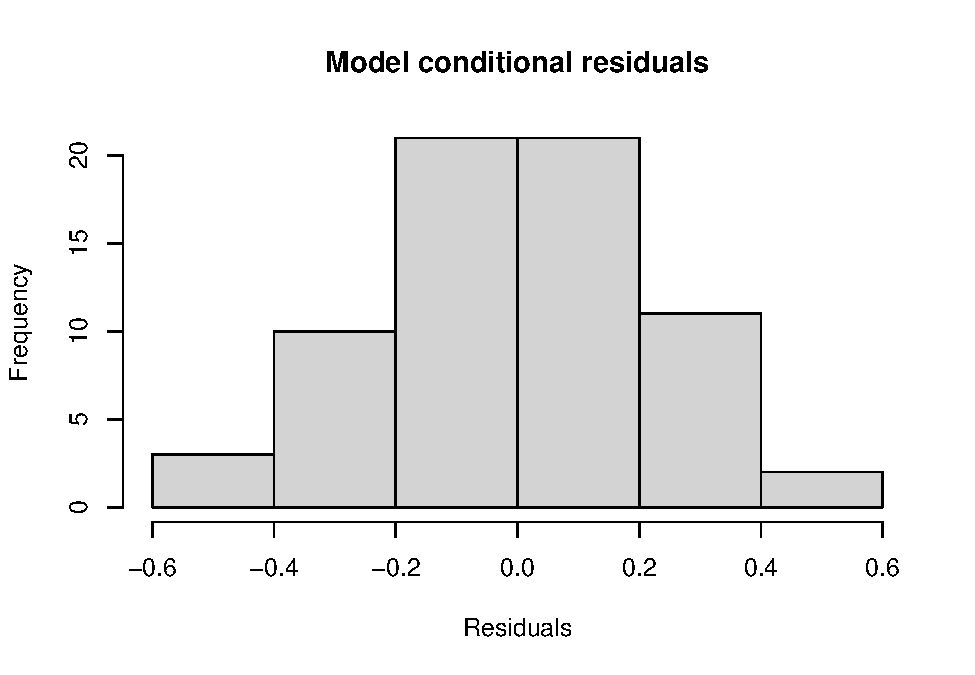
\includegraphics{Supplementary_materials_files/figure-latex/unnamed-chunk-37-1} 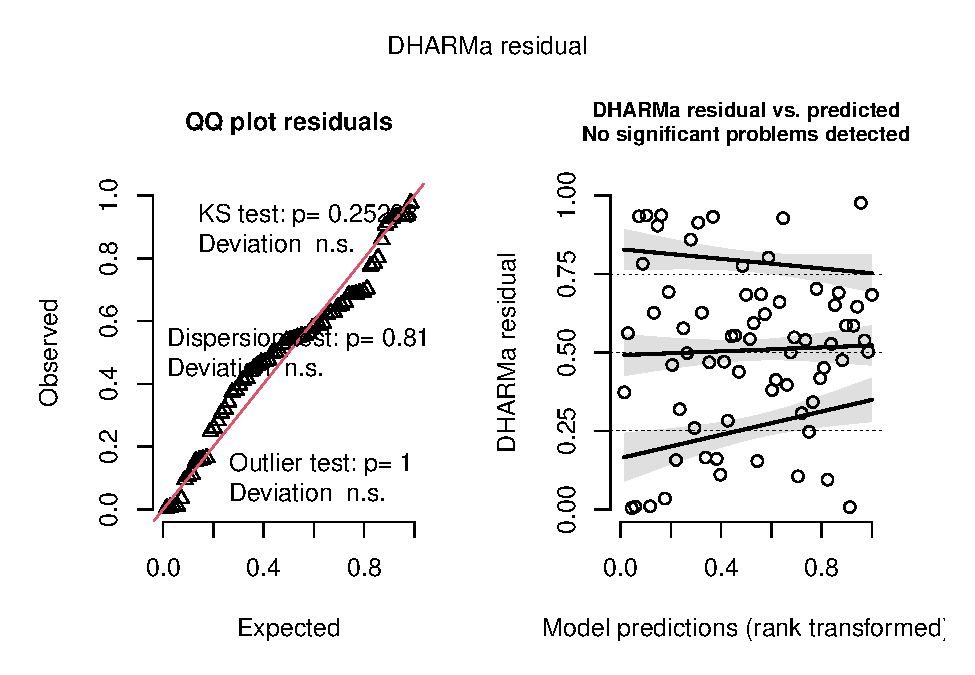
\includegraphics{Supplementary_materials_files/figure-latex/unnamed-chunk-37-2} \end{center}

The model shows no significant effect of body size on CHC amount in \emph{F. sanguinea}, and this term will therefore be excluded from subsequent models for this species.

\subsubsection{\texorpdfstring{\emph{F. fusca}}{F. fusca}}\label{f.-fusca-1}

\[
\log(\text{CHC_mass_fusca}) =  \beta_0 + \text{sanguinea_proportion}+(\text{head_width})^2 + (1|\text{colony_ID}) + \epsilon,
\]
where \(\text{CHC_mass_fusca}\) denotes the total normalized CHC mass on the body of adult \emph{F. fusca} worker.

\begin{verbatim}
## Linear mixed model fit by REML. t-tests use Satterthwaite's method ['lmerModLmerTest']
## Formula: I(log(corrected_mass)) ~ sang_prop + I(head_width^2) + (1 | colony)
##    Data: model_input
## 
## REML criterion at convergence: 127.1
## 
## Scaled residuals: 
##     Min      1Q  Median      3Q     Max 
## -2.7162 -0.5731 -0.1218  0.5782  2.4978 
## 
## Random effects:
##  Groups   Name        Variance Std.Dev.
##  colony   (Intercept) 0.05605  0.2367  
##  Residual             0.16466  0.4058  
## Number of obs: 78, groups:  colony, 20
## 
## Fixed effects:
##                   Estimate Std. Error         df t value Pr(>|t|)    
## (Intercept)      1.512e+00  3.851e-01  5.802e+01   3.926 0.000232 ***
## sang_prop        2.627e-01  1.738e-01  6.883e+01   1.511 0.135262    
## I(head_width^2) -8.355e-07  3.270e-07  5.972e+01  -2.555 0.013192 *  
## ---
## Signif. codes:  0 '***' 0.001 '**' 0.01 '*' 0.05 '.' 0.1 ' ' 1
## 
## Correlation of Fixed Effects:
##             (Intr) sng_pr
## sang_prop    0.077       
## I(hd_wdt^2) -0.974 -0.210
## fit warnings:
## Some predictor variables are on very different scales: consider rescaling
\end{verbatim}

\begin{verbatim}
## 
##  Shapiro-Wilk normality test
## 
## data:  residuals(lm_model)
## W = 0.99146, p-value = 0.8874
\end{verbatim}

\begin{center}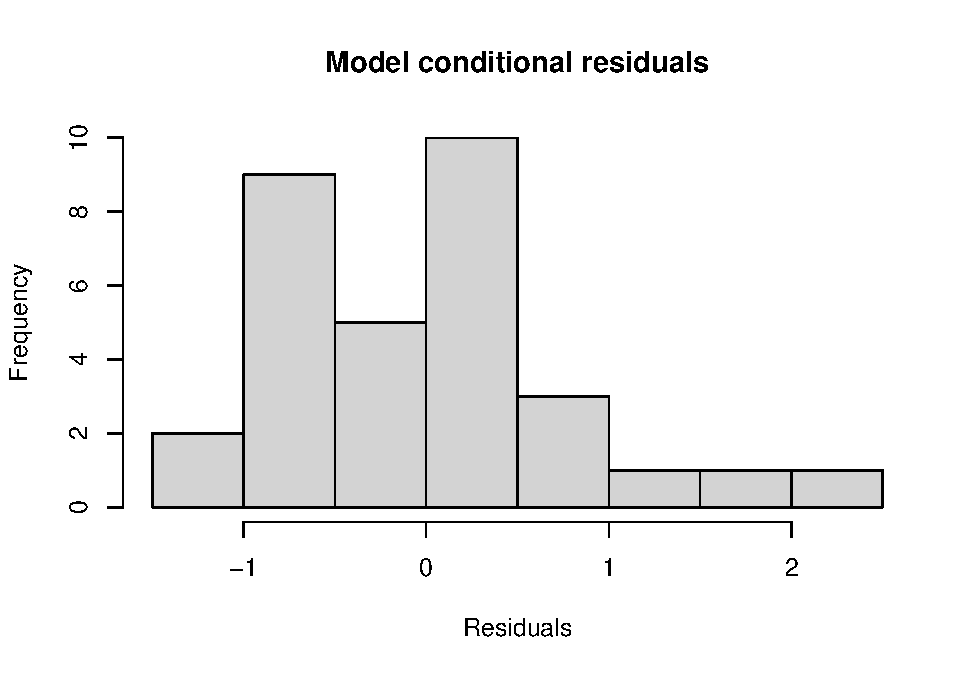
\includegraphics{Supplementary_materials_files/figure-latex/unnamed-chunk-38-1} 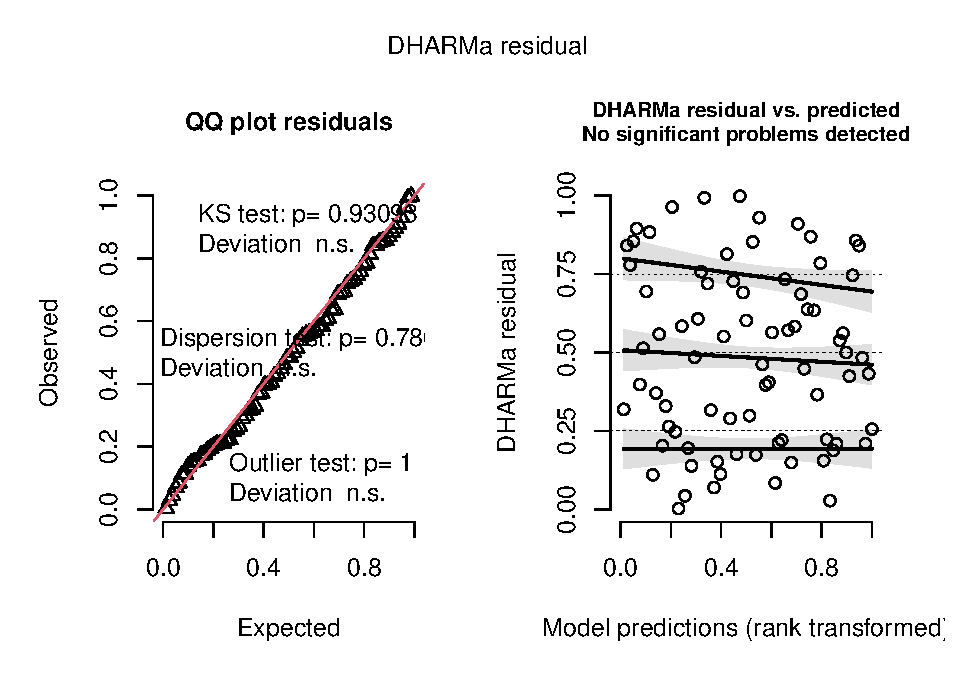
\includegraphics{Supplementary_materials_files/figure-latex/unnamed-chunk-38-2} \end{center}

\subsubsection{\texorpdfstring{Callow \emph{F. sanguinea}}{Callow F. sanguinea}}\label{callow-f.-sanguinea-1}

\[
\log(\text{CHC_mass_callow}) =  \beta_0 + \text{sanguinea_proportion} + (1|\text{colony_ID}) + (1|\text{colony_ID:sampling_occasion_ID}) + \epsilon,
\]
where \(\text{CHC_mass_callow}\) denotes the total normalized CHC mass on the body of callow \emph{F. sanguinea} worker.

\begin{verbatim}
## Linear mixed model fit by REML. t-tests use Satterthwaite's method ['lmerModLmerTest']
## Formula: I(log(corrected_mass)) ~ sang_prop + I(head_width^2) + (1 | colony)
##    Data: model_input
## 
## REML criterion at convergence: 77.4
## 
## Scaled residuals: 
##      Min       1Q   Median       3Q      Max 
## -1.94324 -0.51856  0.06638  0.66444  1.47139 
## 
## Random effects:
##  Groups   Name        Variance Std.Dev.
##  colony   (Intercept) 0.07045  0.2654  
##  Residual             0.21112  0.4595  
## Number of obs: 32, groups:  colony, 16
## 
## Fixed effects:
##                   Estimate Std. Error         df t value Pr(>|t|)   
## (Intercept)      5.190e-01  5.136e-01  2.893e+01   1.010  0.32071   
## sang_prop        1.042e+00  2.968e-01  2.431e+01   3.510  0.00177 **
## I(head_width^2) -4.705e-07  2.899e-07  2.808e+01  -1.623  0.11576   
## ---
## Signif. codes:  0 '***' 0.001 '**' 0.01 '*' 0.05 '.' 0.1 ' ' 1
## 
## Correlation of Fixed Effects:
##             (Intr) sng_pr
## sang_prop   -0.295       
## I(hd_wdt^2) -0.945  0.047
## fit warnings:
## Some predictor variables are on very different scales: consider rescaling
\end{verbatim}

\begin{verbatim}
## 
##  Shapiro-Wilk normality test
## 
## data:  residuals(lm_model)
## W = 0.95837, p-value = 0.2478
\end{verbatim}

\begin{center}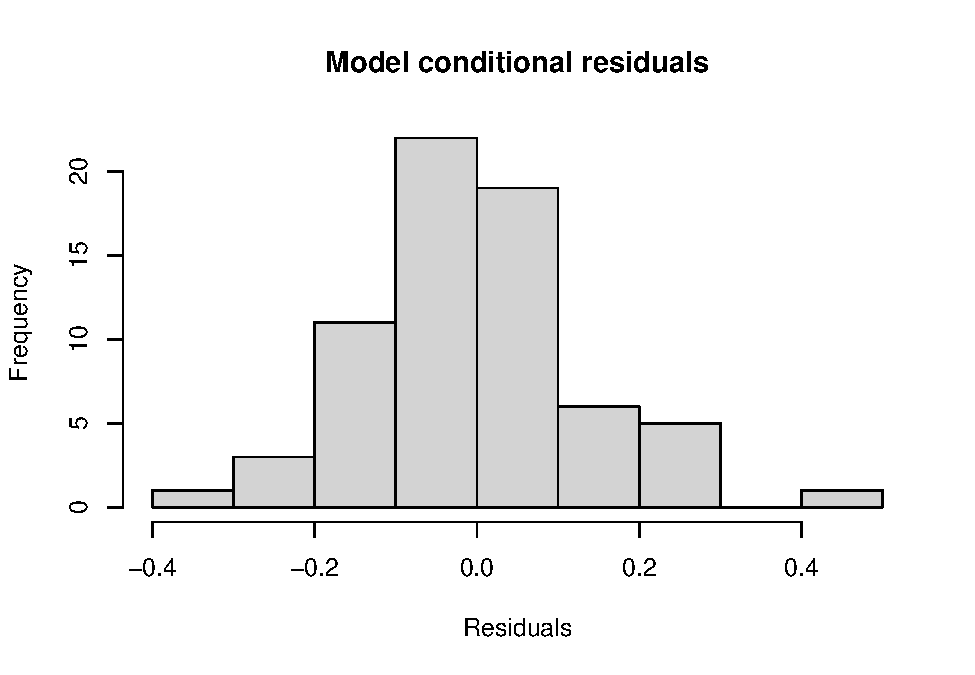
\includegraphics{Supplementary_materials_files/figure-latex/unnamed-chunk-39-1} 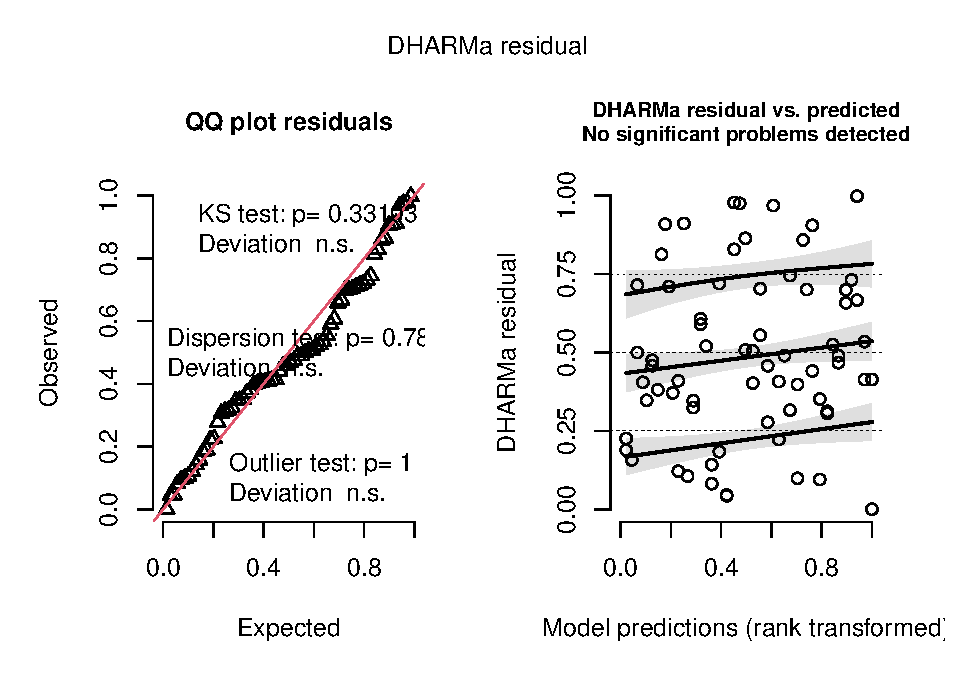
\includegraphics{Supplementary_materials_files/figure-latex/unnamed-chunk-39-2} \end{center}

Similarly to mature \emph{F. sanguinea} ants, in callow workers there is negative but not significant relationship between body size and normalized CHC amount.

\subsection{\texorpdfstring{Change of the CHCs associated with \emph{F. sanguinea}}{Change of the CHCs associated with F. sanguinea}}\label{change-of-the-chcs-associated-with-f.-sanguinea}

In this section the subset of peaks were used to calculate normalized CHC mass. These were peaks identified as \emph{F. sanguinea} markers.

\subsubsection{\texorpdfstring{Mature \emph{F. sanguinea} ants}{Mature F. sanguinea ants}}\label{mature-f.-sanguinea-ants}

\[
\log(\text{CHC_mass_mature}) =  \beta_0 + \text{sanguinea_proportion} + (1|\text{colony_ID}) + (1|\text{colony_ID:sampling_occasion_ID}) + \epsilon,
\]
where \(\text{CHC_mass_mature}\) denotes the normalized mass of \emph{F. sanguinea} markers on the body of adult \emph{F. sanguinea} worker.

\begin{verbatim}
## Linear mixed model fit by REML. t-tests use Satterthwaite's method ['lmerModLmerTest']
## Formula: I(log(corrected_mass + 1)) ~ sang_prop + (1 | colony:census_date) +      (1 | colony)
##    Data: model_input
## 
## REML criterion at convergence: 18.6
## 
## Scaled residuals: 
##      Min       1Q   Median       3Q      Max 
## -1.98685 -0.36446 -0.07957  0.39465  2.48253 
## 
## Random effects:
##  Groups             Name        Variance  Std.Dev. 
##  colony:census_date (Intercept) 5.306e-02 2.303e-01
##  colony             (Intercept) 9.400e-18 3.066e-09
##  Residual                       3.235e-02 1.799e-01
## Number of obs: 68, groups:  colony:census_date, 44; colony, 16
## 
## Fixed effects:
##             Estimate Std. Error       df t value Pr(>|t|)    
## (Intercept)  0.22642    0.07296 40.08019   3.103   0.0035 ** 
## sang_prop    1.16264    0.14177 39.52578   8.201 4.62e-10 ***
## ---
## Signif. codes:  0 '***' 0.001 '**' 0.01 '*' 0.05 '.' 0.1 ' ' 1
## 
## Correlation of Fixed Effects:
##           (Intr)
## sang_prop -0.823
## optimizer (nloptwrap) convergence code: 0 (OK)
## boundary (singular) fit: see help('isSingular')
\end{verbatim}

\begin{verbatim}
## 
##  Shapiro-Wilk normality test
## 
## data:  residuals(lm_model)
## W = 0.97834, p-value = 0.2833
\end{verbatim}

\begin{center}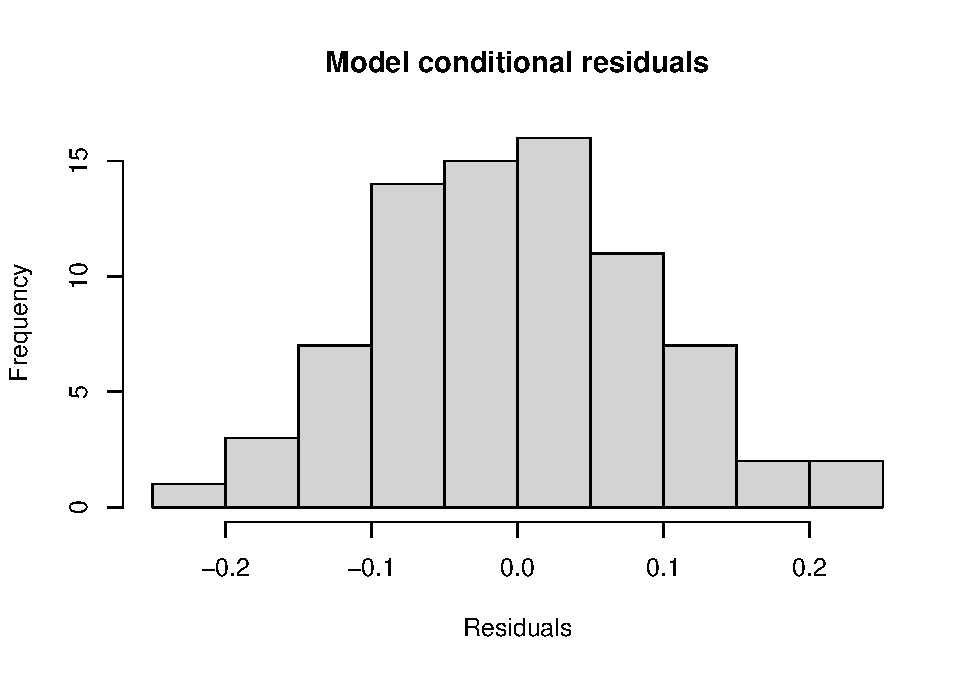
\includegraphics{Supplementary_materials_files/figure-latex/unnamed-chunk-40-1} 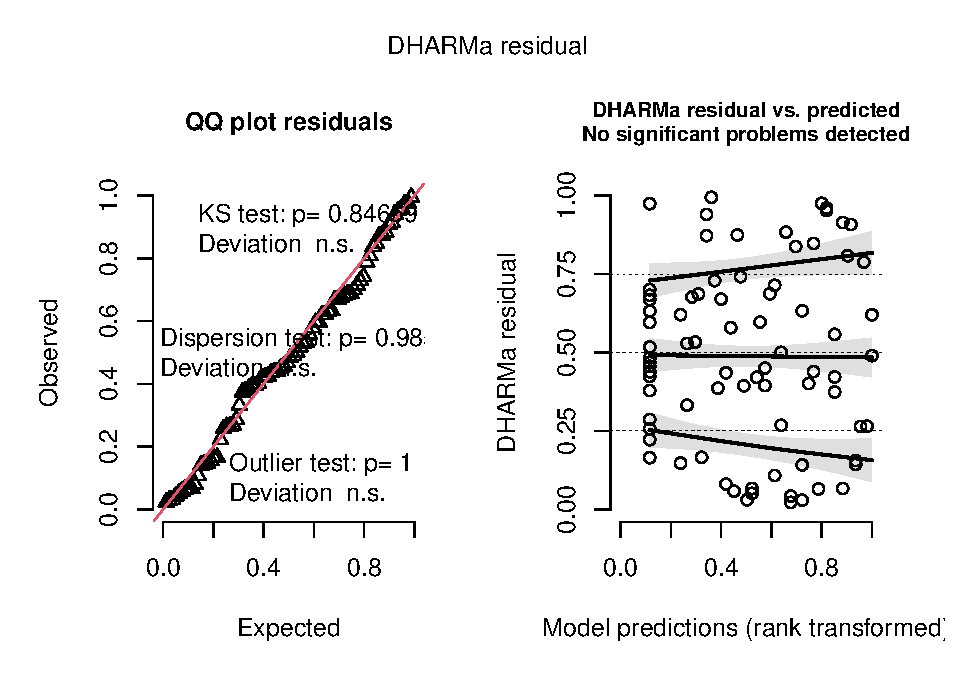
\includegraphics{Supplementary_materials_files/figure-latex/unnamed-chunk-40-2} \end{center}

\subsubsection{\texorpdfstring{\emph{F. fusca} ants}{F. fusca ants}}\label{f.-fusca-ants}

\[
\sqrt{(\text{CHC_mass_fusca})} =  \beta_0 + \text{sanguinea_proportion} +\text{head_width}^2+ (1|\text{colony_ID}) + (1|\text{colony_ID:sampling_occasion_ID}) + \epsilon,
\]
where \(\text{CHC_mass_fusca}\) denotes the normalized mass of \emph{F. sanguinea} markers on the body of adult \emph{F. sanguinea} worker.

\begin{verbatim}
## Linear mixed model fit by REML. t-tests use Satterthwaite's method ['lmerModLmerTest']
## Formula: I(sqrt(corrected_mass)) ~ sang_prop + I(head_width^2) + (1 |      colony:census_date)
##    Data: model_input
## 
## REML criterion at convergence: -40.8
## 
## Scaled residuals: 
##      Min       1Q   Median       3Q      Max 
## -1.83082 -0.49661  0.03171  0.44788  1.87489 
## 
## Random effects:
##  Groups             Name        Variance Std.Dev.
##  colony:census_date (Intercept) 0.009894 0.09947 
##  Residual                       0.013089 0.11441 
## Number of obs: 78, groups:  colony:census_date, 55
## 
## Fixed effects:
##                   Estimate Std. Error         df t value Pr(>|t|)    
## (Intercept)      5.795e-01  1.187e-01  6.889e+01   4.884 6.49e-06 ***
## sang_prop        5.493e-01  6.715e-02  5.172e+01   8.180 6.87e-11 ***
## I(head_width^2) -1.603e-07  1.006e-07  6.993e+01  -1.594    0.116    
## ---
## Signif. codes:  0 '***' 0.001 '**' 0.01 '*' 0.05 '.' 0.1 ' ' 1
## 
## Correlation of Fixed Effects:
##             (Intr) sng_pr
## sang_prop    0.052       
## I(hd_wdt^2) -0.972 -0.224
## fit warnings:
## Some predictor variables are on very different scales: consider rescaling
\end{verbatim}

\begin{verbatim}
## 
##  Shapiro-Wilk normality test
## 
## data:  residuals(lm_model)
## W = 0.98669, p-value = 0.596
\end{verbatim}

\begin{center}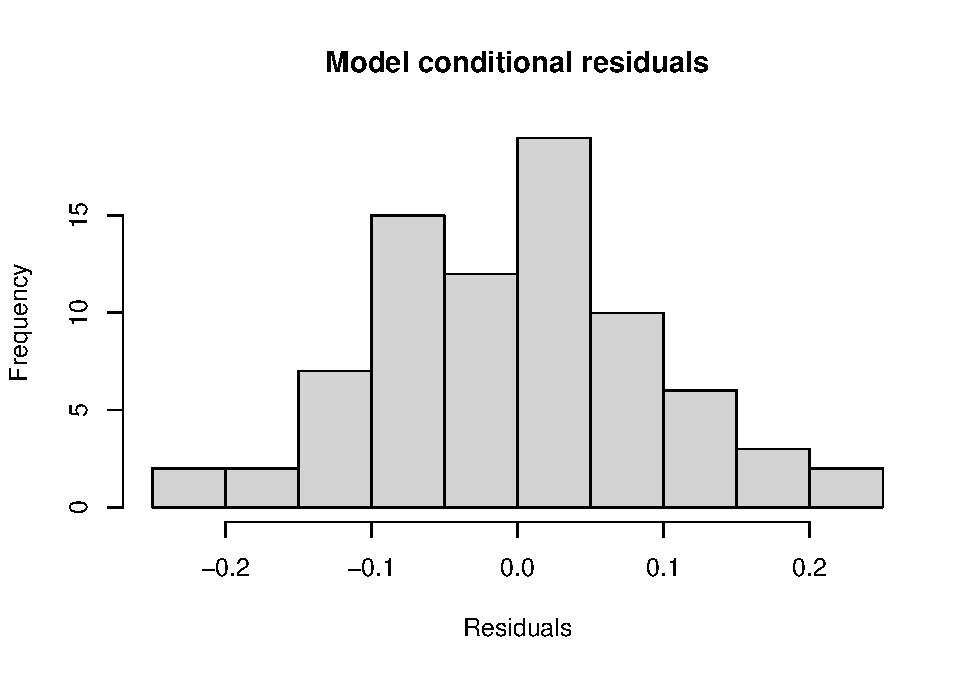
\includegraphics{Supplementary_materials_files/figure-latex/unnamed-chunk-41-1} 
\includegraphics{Supplementary_materials_files/figure-latex/unnamed-chunk-41-2} \end{center}

\subsubsection{\texorpdfstring{Callow \emph{F. sanguinea} ants}{Callow F. sanguinea ants}}\label{callow-f.-sanguinea-ants}

\[
\sqrt[3]{(\text{CHC_mass_mature})} = \beta_0 + \text{sanguinea_proportion} + \epsilon,
\]
where \(\text{CHC_mass_mature}\) denotes the normalized mass of \emph{F. sanguinea} markers on the body of callow \emph{F. sanguinea} worker.

\begin{verbatim}
## 
## Call:
## lm(formula = I((corrected_mass)^(1/3)) ~ sang_prop, data = model_input)
## 
## Residuals:
##      Min       1Q   Median       3Q      Max 
## -0.37888 -0.07244  0.02268  0.08319  0.30937 
## 
## Coefficients:
##             Estimate Std. Error t value Pr(>|t|)    
## (Intercept)  0.29848    0.04202   7.104  6.7e-08 ***
## sang_prop    0.63173    0.07899   7.998  6.3e-09 ***
## ---
## Signif. codes:  0 '***' 0.001 '**' 0.01 '*' 0.05 '.' 0.1 ' ' 1
## 
## Residual standard error: 0.1335 on 30 degrees of freedom
## Multiple R-squared:  0.6807, Adjusted R-squared:  0.6701 
## F-statistic: 63.96 on 1 and 30 DF,  p-value: 6.305e-09
\end{verbatim}

\begin{verbatim}
## 
##  Shapiro-Wilk normality test
## 
## data:  residuals(lm_model)
## W = 0.96975, p-value = 0.4925
\end{verbatim}

\begin{center}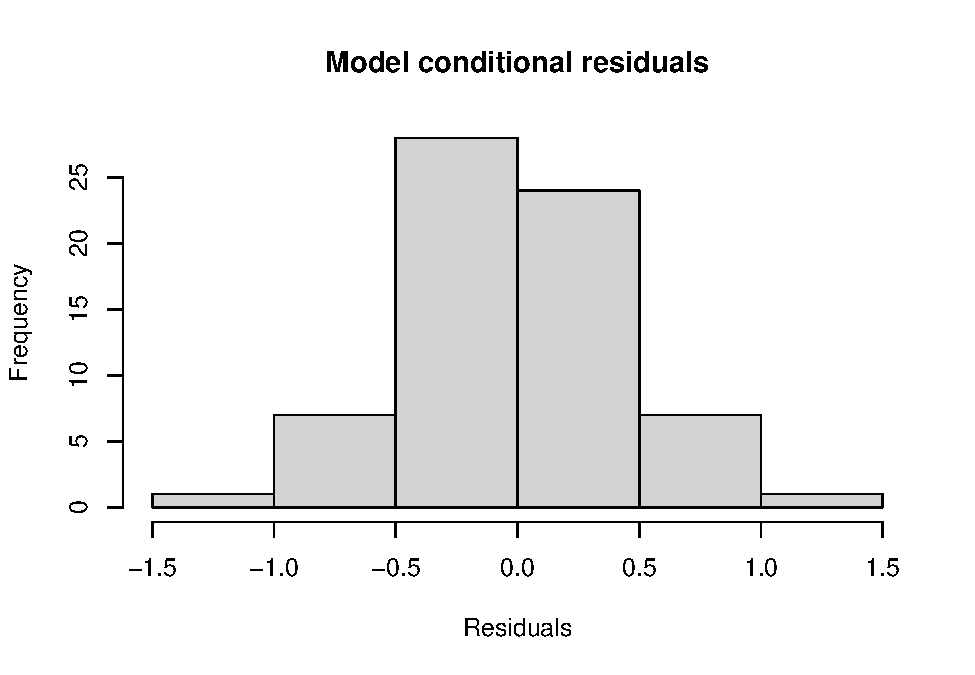
\includegraphics{Supplementary_materials_files/figure-latex/unnamed-chunk-42-1} \end{center}

\subsection{\texorpdfstring{Change of the CHCs associated with \emph{F. fusca}}{Change of the CHCs associated with F. fusca}}\label{change-of-the-chcs-associated-with-f.-fusca}

Similarly to the analysis with the use of markers of \emph{F. sanguinea} workers, the procedure was repeated using the mass of \emph{F. fusca} markers as a response variable.

\subsubsection{\texorpdfstring{Mature \emph{F. sanguinea} ants}{Mature F. sanguinea ants}}\label{mature-f.-sanguinea-ants-1}

\[
\log(\text{CHC_mass_mature}) =  \beta_0 + \text{sanguinea_proportion} + (1|\text{colony_ID}) + (1|\text{colony_ID:sampling_occasion_ID}) + \epsilon,
\]
where \(\text{CHC_mass_mature}\) denotes the normalized mass of \emph{F. fusca} markers on the body of adult \emph{F. sanguinea} worker.

\begin{verbatim}
## Linear mixed model fit by REML. t-tests use Satterthwaite's method ['lmerModLmerTest']
## Formula: I(log(corrected_mass)) ~ sang_prop + (1 | colony:census_date) +      (1 | colony)
##    Data: model_input
## 
## REML criterion at convergence: 154.6
## 
## Scaled residuals: 
##      Min       1Q   Median       3Q      Max 
## -2.32675 -0.47439 -0.04918  0.42137  2.01162 
## 
## Random effects:
##  Groups             Name        Variance Std.Dev.
##  colony:census_date (Intercept) 0.1184   0.3442  
##  colony             (Intercept) 0.3702   0.6084  
##  Residual                       0.3039   0.5513  
## Number of obs: 68, groups:  colony:census_date, 44; colony, 16
## 
## Fixed effects:
##             Estimate Std. Error      df t value Pr(>|t|)    
## (Intercept)  -0.5686     0.2268 31.9619  -2.507   0.0174 *  
## sang_prop    -1.8817     0.3262 30.8622  -5.769 2.41e-06 ***
## ---
## Signif. codes:  0 '***' 0.001 '**' 0.01 '*' 0.05 '.' 0.1 ' ' 1
## 
## Correlation of Fixed Effects:
##           (Intr)
## sang_prop -0.626
\end{verbatim}

\begin{verbatim}
## 
##  Shapiro-Wilk normality test
## 
## data:  residuals(lm_model)
## W = 0.98815, p-value = 0.7693
\end{verbatim}

\begin{center}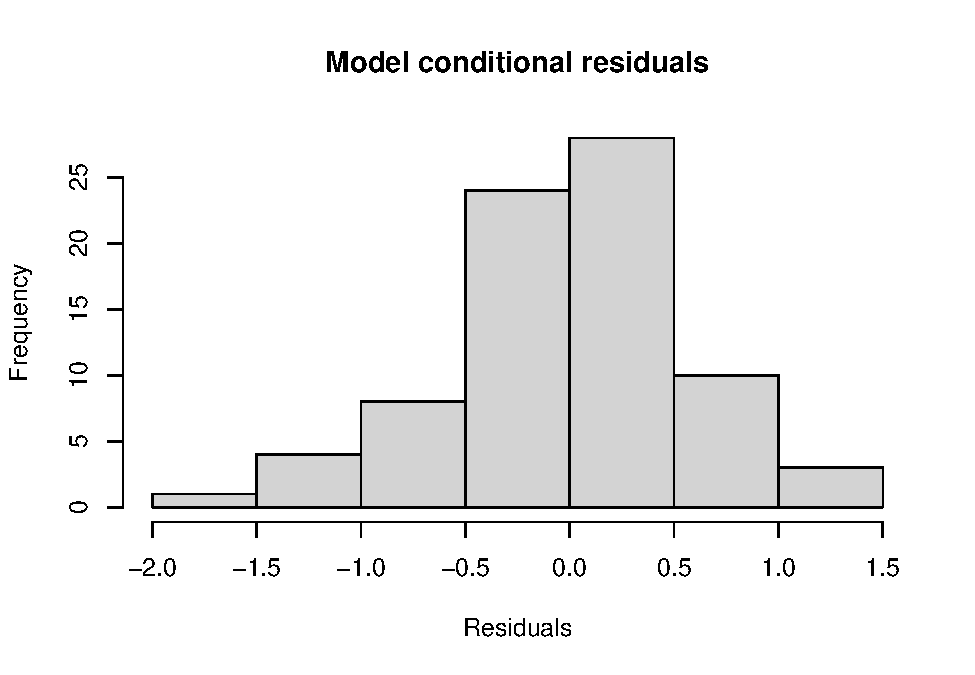
\includegraphics{Supplementary_materials_files/figure-latex/unnamed-chunk-43-1} 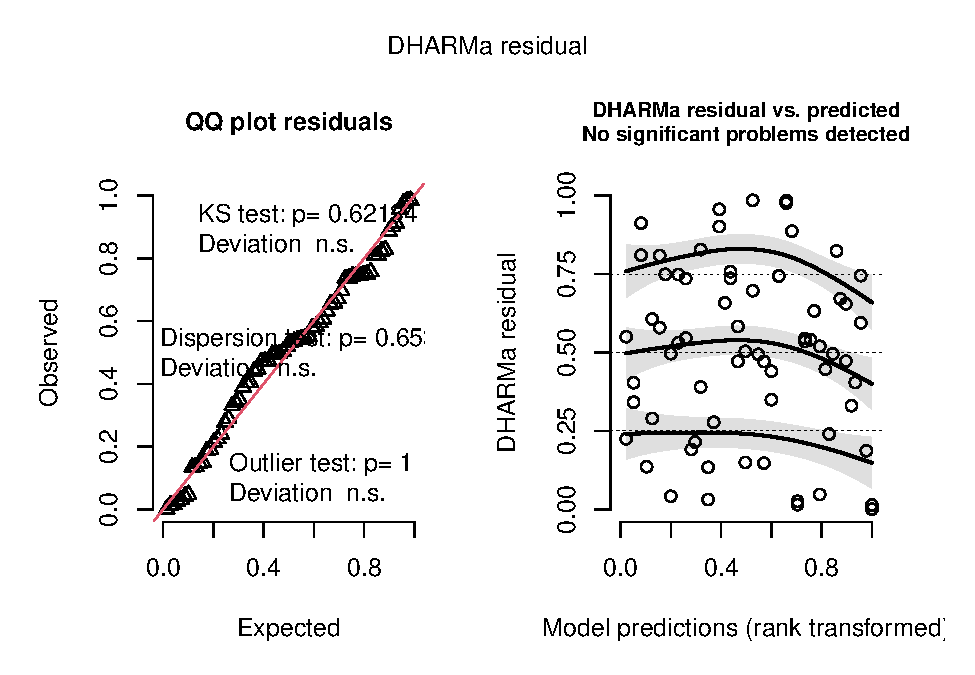
\includegraphics{Supplementary_materials_files/figure-latex/unnamed-chunk-43-2} \end{center}

\subsubsection{\texorpdfstring{\emph{F. fusca} ants}{F. fusca ants}}\label{f.-fusca-ants-1}

\[
\log(\text{CHC_mass_mature}+0.01) =  \beta_0 + \text{sanguinea_proportion} + \text{head_width}^2+(1|\text{colony_ID}) + (1|\text{colony_ID:sampling_occasion_ID}) + \epsilon,
\]
where \(\text{CHC_mass_mature}\) denotes the normalized mass of \emph{F. fusca} markers on the body of \emph{F. fusca} worker.

\begin{verbatim}
## Linear mixed model fit by REML. t-tests use Satterthwaite's method ['lmerModLmerTest']
## Formula: I(log(corrected_mass + 0.01)) ~ sang_prop + I(head_width^2) +  
##     (1 | colony) + (1 | colony:census_date)
##    Data: model_input
## 
## REML criterion at convergence: 198.3
## 
## Scaled residuals: 
##      Min       1Q   Median       3Q      Max 
## -2.56390 -0.62519  0.05594  0.58570  2.25157 
## 
## Random effects:
##  Groups             Name        Variance  Std.Dev. 
##  colony:census_date (Intercept) 6.104e-10 2.471e-05
##  colony             (Intercept) 2.590e-01 5.089e-01
##  Residual                       3.830e-01 6.188e-01
## Number of obs: 78, groups:  colony:census_date, 55; colony, 20
## 
## Fixed effects:
##                   Estimate Std. Error         df t value Pr(>|t|)    
## (Intercept)      1.913e-03  6.383e-01  7.162e+01   0.003   0.9976    
## sang_prop       -1.367e+00  2.715e-01  6.631e+01  -5.034 3.93e-06 ***
## I(head_width^2) -9.525e-07  5.398e-07  7.330e+01  -1.765   0.0818 .  
## ---
## Signif. codes:  0 '***' 0.001 '**' 0.01 '*' 0.05 '.' 0.1 ' ' 1
## 
## Correlation of Fixed Effects:
##             (Intr) sng_pr
## sang_prop    0.088       
## I(hd_wdt^2) -0.969 -0.212
## fit warnings:
## Some predictor variables are on very different scales: consider rescaling
## optimizer (nloptwrap) convergence code: 0 (OK)
## boundary (singular) fit: see help('isSingular')
\end{verbatim}

\begin{verbatim}
## 
##  Shapiro-Wilk normality test
## 
## data:  residuals(lm_model)
## W = 0.98552, p-value = 0.5236
\end{verbatim}

\begin{center}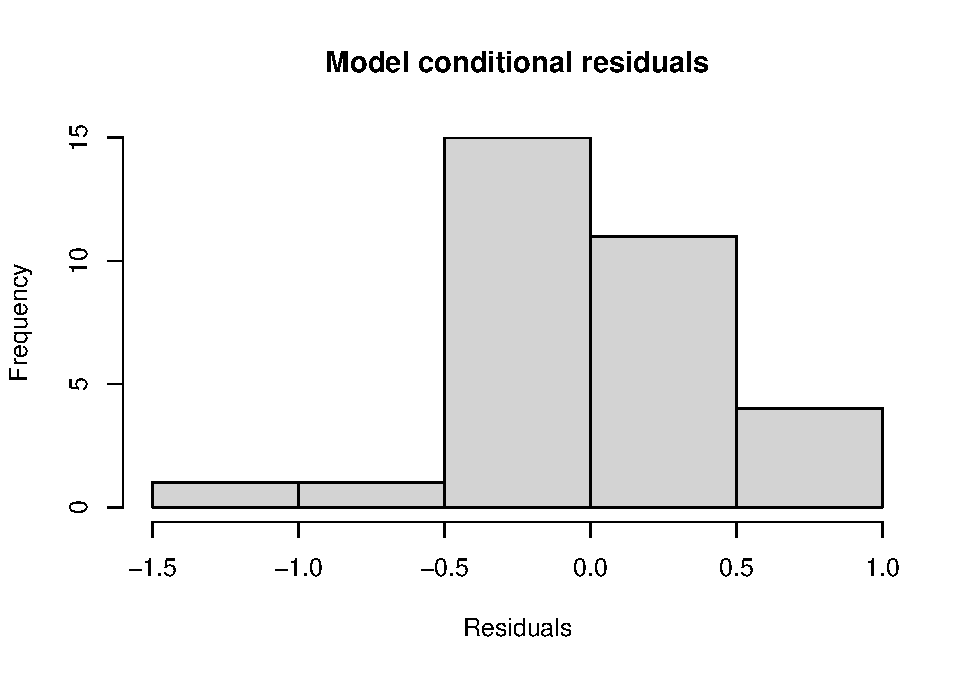
\includegraphics{Supplementary_materials_files/figure-latex/unnamed-chunk-44-1} \includegraphics{Supplementary_materials_files/figure-latex/unnamed-chunk-44-2} \end{center}

\subsubsection{\texorpdfstring{Callow \emph{F. sanguinea} ants}{Callow F. sanguinea ants}}\label{callow-f.-sanguinea-ants-1}

\[
\log(\text{CHC_mass_mature}) = \beta_0 + \text{sanguinea_proportion} + (1|\text{colony_ID}) + \epsilon,
\]
where \(\log(\text{CHC_mass_mature})\) denotes the normalized mass of \emph{F. fusca} markers on the body of callow \emph{F. sanguinea} worker.

\begin{verbatim}
## Linear mixed model fit by REML. t-tests use Satterthwaite's method ['lmerModLmerTest']
## Formula: I(log(corrected_mass)) ~ sang_prop + (1 | colony)
##    Data: model_input
## 
## REML criterion at convergence: 64.7
## 
## Scaled residuals: 
##      Min       1Q   Median       3Q      Max 
## -2.29425 -0.57286 -0.03774  0.61675  1.83684 
## 
## Random effects:
##  Groups   Name        Variance Std.Dev.
##  colony   (Intercept) 0.2338   0.4835  
##  Residual             0.2733   0.5228  
## Number of obs: 32, groups:  colony, 16
## 
## Fixed effects:
##             Estimate Std. Error      df t value Pr(>|t|)    
## (Intercept)  -1.9565     0.2187 28.3341  -8.944 9.58e-10 ***
## sang_prop    -0.1866     0.3551 20.4211  -0.525    0.605    
## ---
## Signif. codes:  0 '***' 0.001 '**' 0.01 '*' 0.05 '.' 0.1 ' ' 1
## 
## Correlation of Fixed Effects:
##           (Intr)
## sang_prop -0.700
\end{verbatim}

\begin{verbatim}
## 
##  Shapiro-Wilk normality test
## 
## data:  residuals(lm_model)
## W = 0.97969, p-value = 0.7905
\end{verbatim}

\begin{center}
\includegraphics{Supplementary_materials_files/figure-latex/unnamed-chunk-45-1} \end{center}

\section{Comparison of the amount and proportions of CHC between species and age categories}\label{comparison-of-the-amount-and-proportions-of-chc-between-species-and-age-categories}

This section presents the results of Wilcoxon tests comparing features of CHC profiles between callow and mature \emph{F. sanguinea} ants as well as \emph{F. fusca} slaves. Samples from the same colony were averaged before calculation of the final statistics to account for their non-independence.

\subsection{\texorpdfstring{Difference in the total CHC amount between \emph{F. sanguinea} and \emph{F. fusca}}{Difference in the total CHC amount between F. sanguinea and F. fusca}}\label{difference-in-the-total-chc-amount-between-f.-sanguinea-and-f.-fusca}

\begin{verbatim}
## # A tibble: 1 x 7
##   .y.            group1   group2         n1    n2 statistic       p
## * <chr>          <chr>    <chr>       <int> <int>     <dbl>   <dbl>
## 1 corrected_mass F. fusca F. sanginea    16    16         7 0.00058
\end{verbatim}

\begin{center}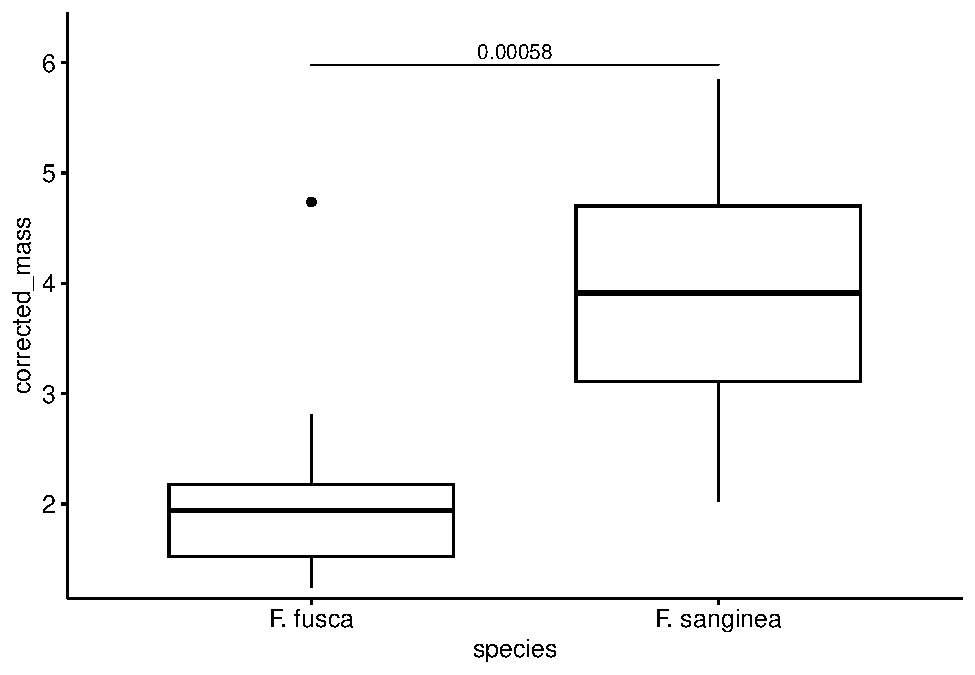
\includegraphics{Supplementary_materials_files/figure-latex/unnamed-chunk-47-1} \end{center}

\subsection{\texorpdfstring{Difference in the total CHC amount between callow and mature \emph{F. sanguinea}}{Difference in the total CHC amount between callow and mature F. sanguinea}}\label{difference-in-the-total-chc-amount-between-callow-and-mature-f.-sanguinea}

\begin{verbatim}
## # A tibble: 1 x 7
##   .y.            group1 group2    n1    n2 statistic         p
## * <chr>          <chr>  <chr>  <int> <int>     <dbl>     <dbl>
## 1 corrected_mass 0      1         16    16       136 0.0000305
\end{verbatim}

\begin{center}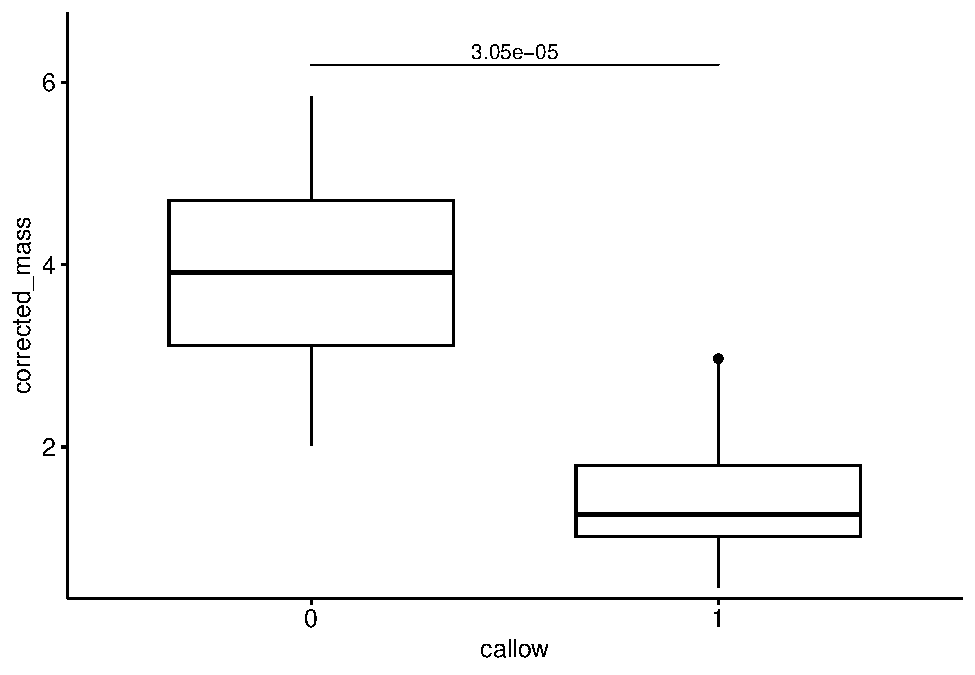
\includegraphics{Supplementary_materials_files/figure-latex/unnamed-chunk-48-1} \end{center}

\subsection{\texorpdfstring{Difference in the proportion of CHC characteristic of \emph{F. sanguinea} between mature \emph{F. sanguinea} and \emph{F. fusca}}{Difference in the proportion of CHC characteristic of F. sanguinea between mature F. sanguinea and F. fusca}}\label{difference-in-the-proportion-of-chc-characteristic-of-f.-sanguinea-between-mature-f.-sanguinea-and-f.-fusca}

\begin{center}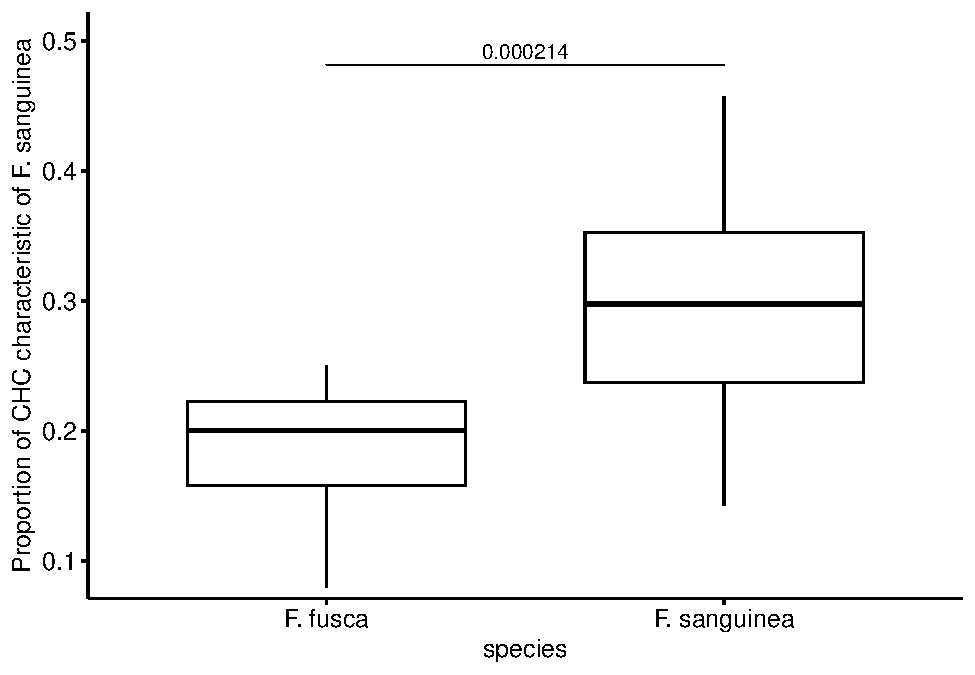
\includegraphics{Supplementary_materials_files/figure-latex/unnamed-chunk-49-1} \end{center}

\subsection{\texorpdfstring{Difference in the proportion of CHC characteristic of \emph{F. sanguinea} between mature and callow \emph{F. sanguinea}}{Difference in the proportion of CHC characteristic of F. sanguinea between mature and callow F. sanguinea}}\label{difference-in-the-proportion-of-chc-characteristic-of-f.-sanguinea-between-mature-and-callow-f.-sanguinea}

\begin{center}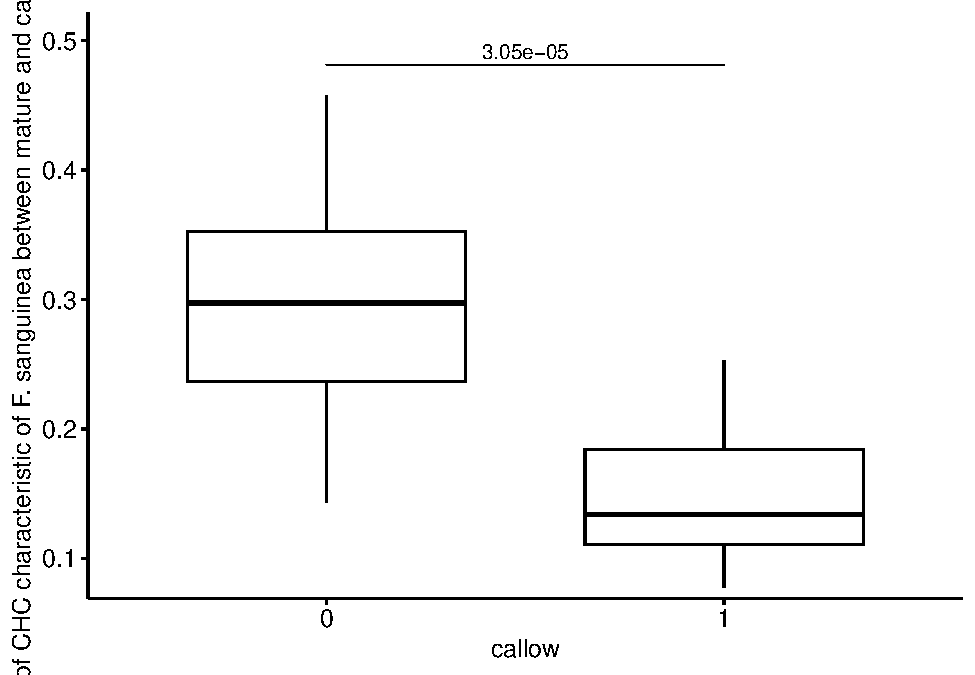
\includegraphics{Supplementary_materials_files/figure-latex/unnamed-chunk-50-1} \end{center}

\subsection{\texorpdfstring{Difference in the proportion of CHC characteristic of callow \emph{F. sanguinea} between mature and callow \emph{F. sanguinea}}{Difference in the proportion of CHC characteristic of callow F. sanguinea between mature and callow F. sanguinea}}\label{difference-in-the-proportion-of-chc-characteristic-of-callow-f.-sanguinea-between-mature-and-callow-f.-sanguinea}

\begin{center}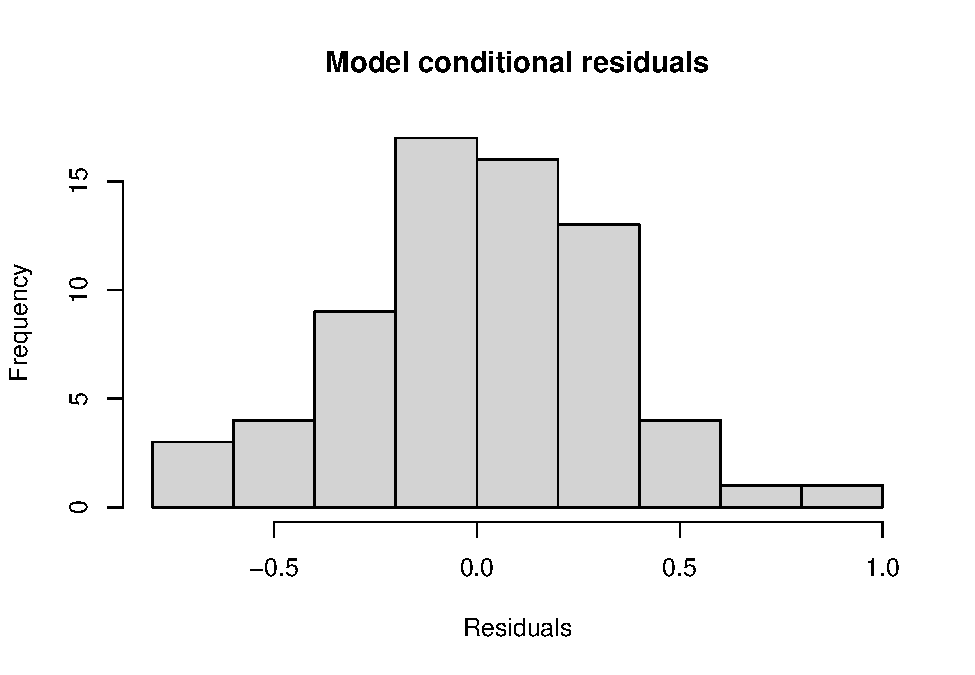
\includegraphics{Supplementary_materials_files/figure-latex/unnamed-chunk-51-1} \end{center}

\subsection{\texorpdfstring{Difference in the amount of CHC characteristic of callow \emph{F. sanguinea} between mature and callow \emph{F. sanguinea}}{Difference in the amount of CHC characteristic of callow F. sanguinea between mature and callow F. sanguinea}}\label{difference-in-the-amount-of-chc-characteristic-of-callow-f.-sanguinea-between-mature-and-callow-f.-sanguinea}

\begin{center}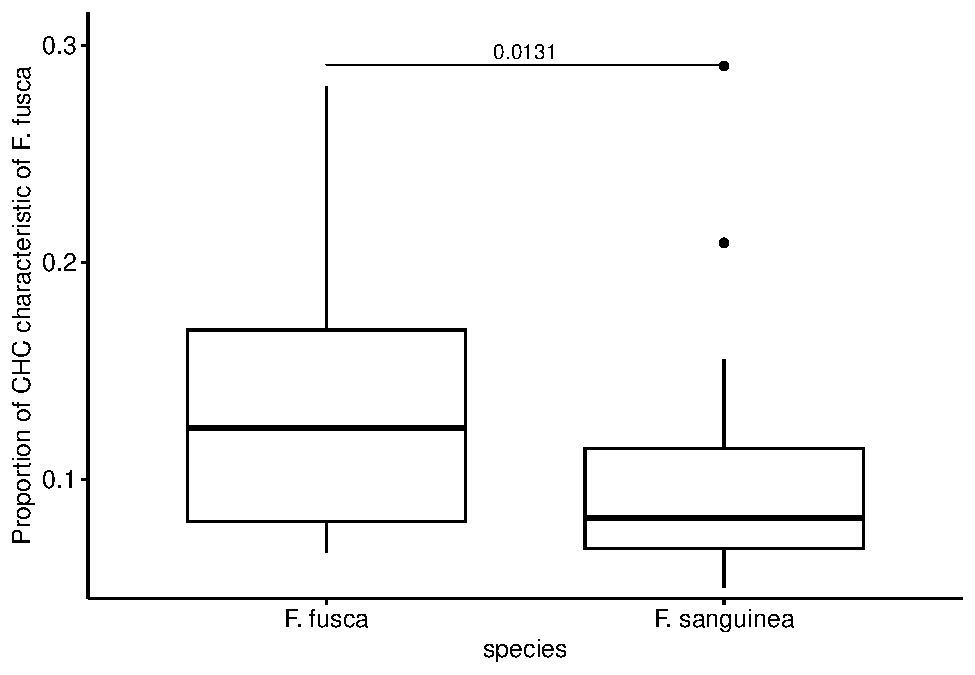
\includegraphics{Supplementary_materials_files/figure-latex/unnamed-chunk-52-1} \end{center}

\subsection{\texorpdfstring{Difference in the proportion of CHC characteristic of \emph{F. fusca} between mature \emph{F. sanguinea} and \emph{F. fusca}}{Difference in the proportion of CHC characteristic of F. fusca between mature F. sanguinea and F. fusca}}\label{difference-in-the-proportion-of-chc-characteristic-of-f.-fusca-between-mature-f.-sanguinea-and-f.-fusca}

\begin{center}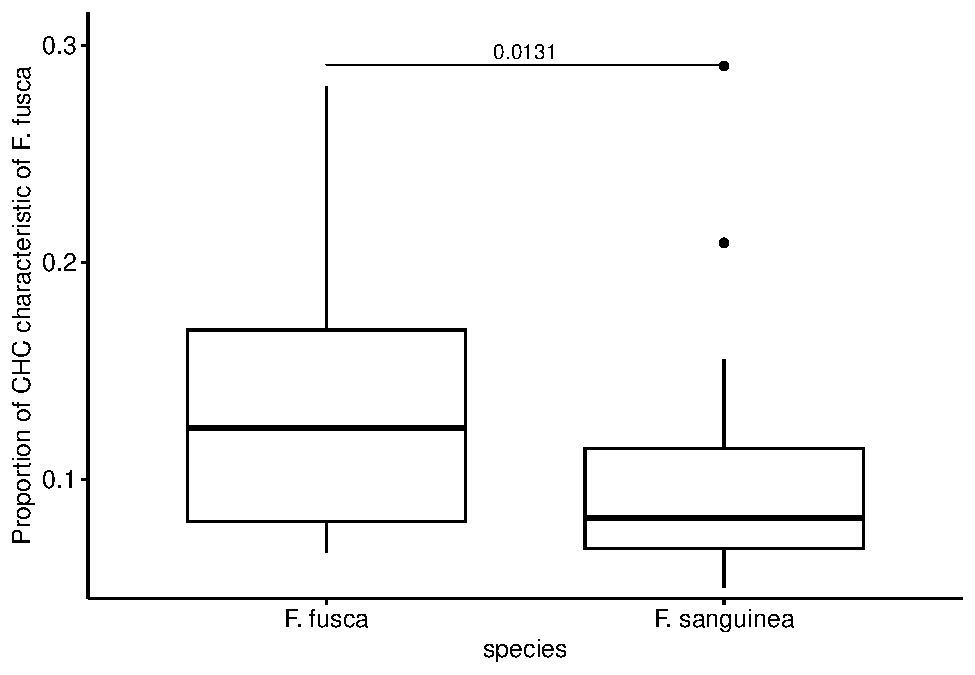
\includegraphics{Supplementary_materials_files/figure-latex/unnamed-chunk-53-1} \end{center}

\subsection{\texorpdfstring{Difference in the proportion of CHC characteristic of \emph{F. fusca} between mature and callow \emph{F. sanguinea}}{Difference in the proportion of CHC characteristic of F. fusca between mature and callow F. sanguinea}}\label{difference-in-the-proportion-of-chc-characteristic-of-f.-fusca-between-mature-and-callow-f.-sanguinea}

\begin{center}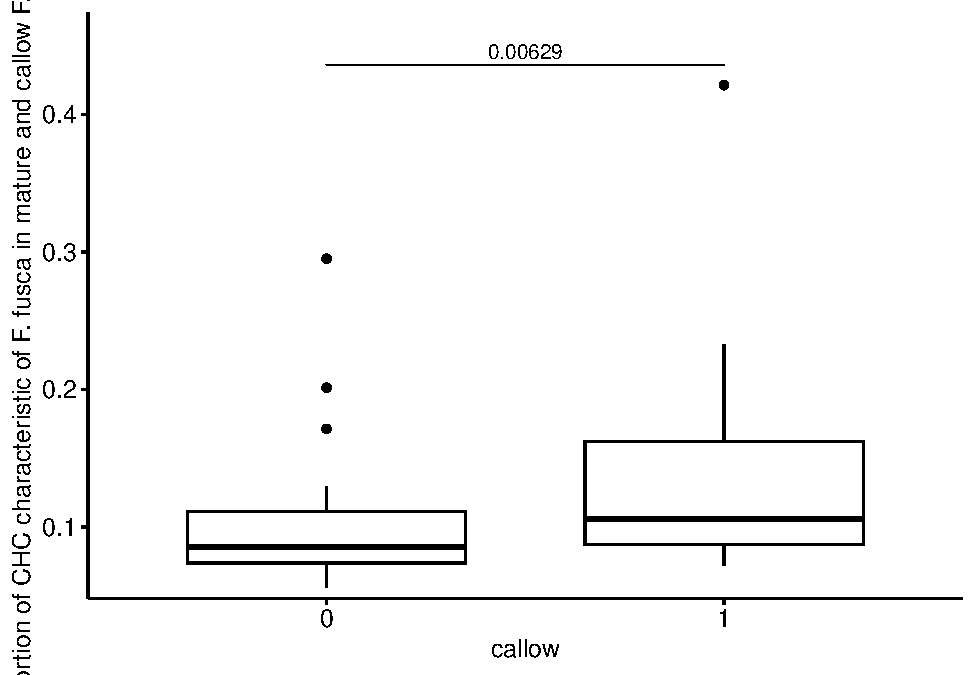
\includegraphics{Supplementary_materials_files/figure-latex/unnamed-chunk-54-1} \end{center}

\subsection{\texorpdfstring{Difference in the proportion of CHC characteristic of \emph{F. fusca} between callow \emph{F. sanguinea} and \emph{F. fusca}}{Difference in the proportion of CHC characteristic of F. fusca between callow F. sanguinea and F. fusca}}\label{difference-in-the-proportion-of-chc-characteristic-of-f.-fusca-between-callow-f.-sanguinea-and-f.-fusca}

\begin{center}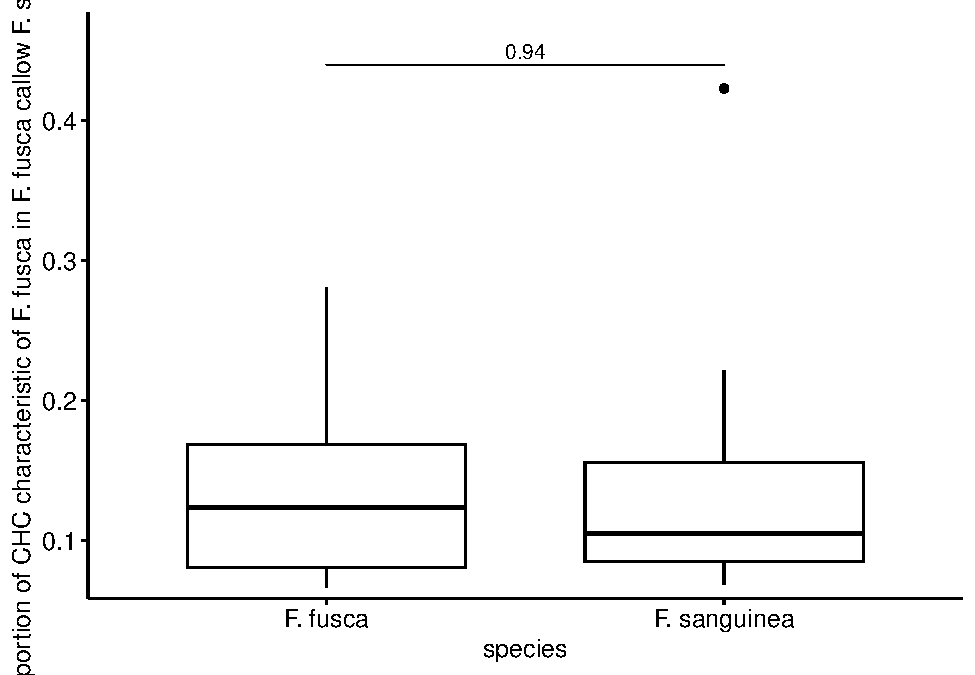
\includegraphics{Supplementary_materials_files/figure-latex/unnamed-chunk-55-1} \end{center}

\subsection{\texorpdfstring{Difference in the mass of \emph{n}-alkanes between callow and mature \emph{F. sanguinea}}{Difference in the mass of n-alkanes between callow and mature F. sanguinea}}\label{difference-in-the-mass-of-n-alkanes-between-callow-and-mature-f.-sanguinea}

\begin{center}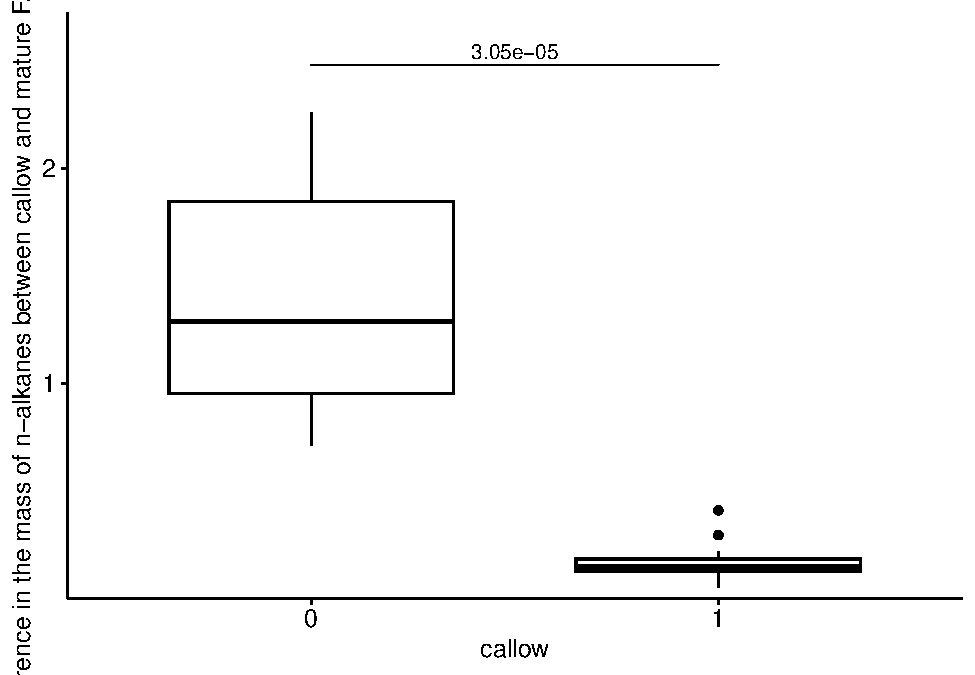
\includegraphics{Supplementary_materials_files/figure-latex/unnamed-chunk-56-1} \end{center}

\subsection{\texorpdfstring{Difference in the proprtion of \emph{n}-alkanes between callow and mature \emph{F. sanguinea}}{Difference in the proprtion of n-alkanes between callow and mature F. sanguinea}}\label{difference-in-the-proprtion-of-n-alkanes-between-callow-and-mature-f.-sanguinea}

\begin{center}
\includegraphics{Supplementary_materials_files/figure-latex/unnamed-chunk-57-1} \end{center}

\section{\texorpdfstring{Change in the CHC profile in separated callow \emph{F. sanguinea} ants}{Change in the CHC profile in separated callow F. sanguinea ants}}\label{change-in-the-chc-profile-in-separated-callow-f.-sanguinea-ants}

\subsection{Change in the total CHC amount over time}\label{change-in-the-total-chc-amount-over-time}

\begin{verbatim}
## Linear mixed model fit by REML. t-tests use Satterthwaite's method ['lmerModLmerTest']
## Formula: I(sqrt(corrected_mass)) ~ mean_delta + (1 | colony)
##    Data: separation_data[-74, ]
## 
## REML criterion at convergence: -12.9
## 
## Scaled residuals: 
##      Min       1Q   Median       3Q      Max 
## -2.54596 -0.65494 -0.04106  0.63627  2.54062 
## 
## Random effects:
##  Groups   Name        Variance Std.Dev.
##  colony   (Intercept) 0.01293  0.1137  
##  Residual             0.03516  0.1875  
## Number of obs: 79, groups:  colony, 11
## 
## Fixed effects:
##              Estimate Std. Error        df t value Pr(>|t|)    
## (Intercept)  1.180332   0.047605 16.450772  24.794 1.83e-14 ***
## mean_delta   0.002458   0.001669 68.538937   1.473    0.145    
## ---
## Signif. codes:  0 '***' 0.001 '**' 0.01 '*' 0.05 '.' 0.1 ' ' 1
## 
## Correlation of Fixed Effects:
##            (Intr)
## mean_delta -0.518
\end{verbatim}

\begin{verbatim}
## 
##  Shapiro-Wilk normality test
## 
## data:  residuals(lm_model)
## W = 0.99204, p-value = 0.9107
\end{verbatim}

\begin{center}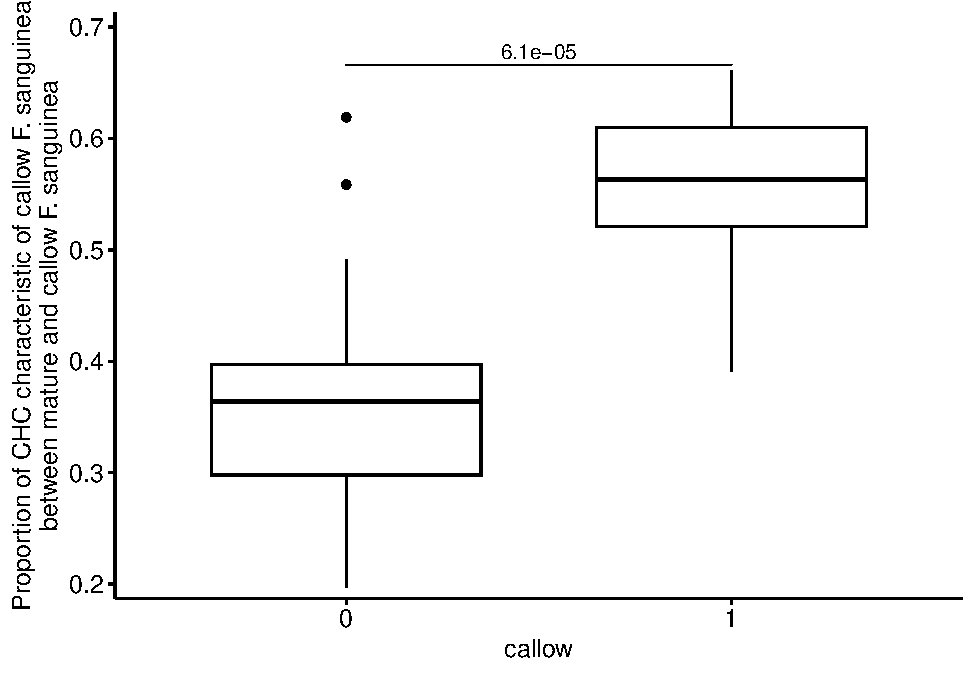
\includegraphics{Supplementary_materials_files/figure-latex/unnamed-chunk-59-1} 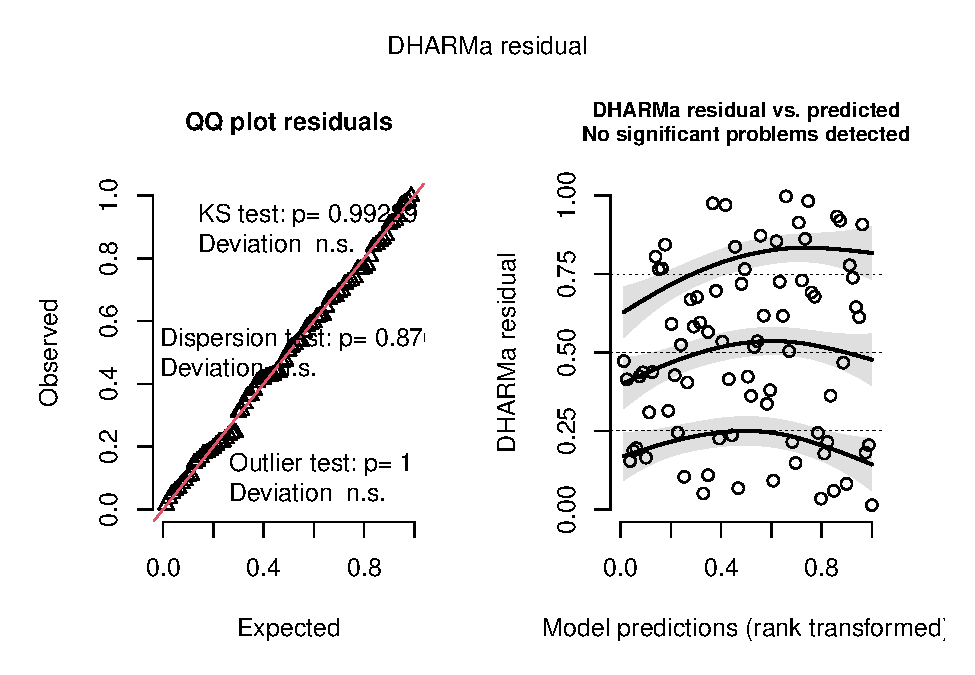
\includegraphics{Supplementary_materials_files/figure-latex/unnamed-chunk-59-2} \end{center}

\subsection{\texorpdfstring{Change in the amount of compounds associated with callow \emph{F. sanguinea}}{Change in the amount of compounds associated with callow F. sanguinea}}\label{change-in-the-amount-of-compounds-associated-with-callow-f.-sanguinea}

\begin{verbatim}
## Linear mixed model fit by REML. t-tests use Satterthwaite's method ['lmerModLmerTest']
## Formula: log(corrected_mass_part) ~ mean_delta + (1 | colony)
##    Data: separation_data
## 
## REML criterion at convergence: 90.5
## 
## Scaled residuals: 
##     Min      1Q  Median      3Q     Max 
## -2.3283 -0.7175  0.1030  0.6844  2.5692 
## 
## Random effects:
##  Groups   Name        Variance Std.Dev.
##  colony   (Intercept) 0.09983  0.3160  
##  Residual             0.12268  0.3503  
## Number of obs: 80, groups:  colony, 11
## 
## Fixed effects:
##              Estimate Std. Error        df t value Pr(>|t|)   
## (Intercept) -0.348801   0.113427 13.345289  -3.075  0.00863 **
## mean_delta  -0.004344   0.003040 68.378442  -1.429  0.15750   
## ---
## Signif. codes:  0 '***' 0.001 '**' 0.01 '*' 0.05 '.' 0.1 ' ' 1
## 
## Correlation of Fixed Effects:
##            (Intr)
## mean_delta -0.405
\end{verbatim}

\begin{verbatim}
## 
##  Shapiro-Wilk normality test
## 
## data:  residuals(lm_model)
## W = 0.99175, p-value = 0.8938
\end{verbatim}

\begin{center}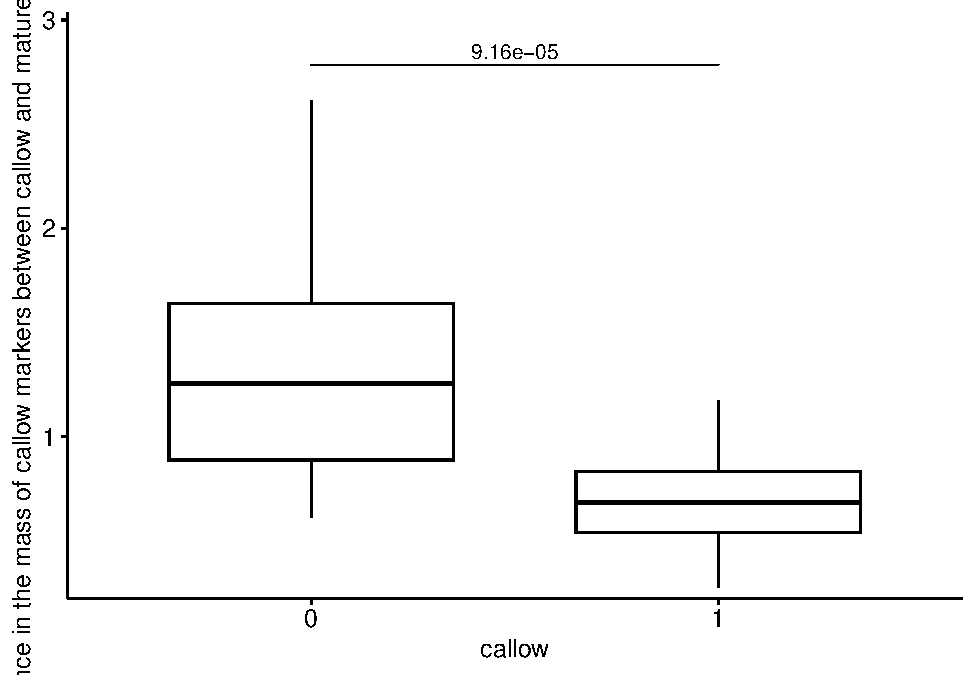
\includegraphics{Supplementary_materials_files/figure-latex/unnamed-chunk-60-1} 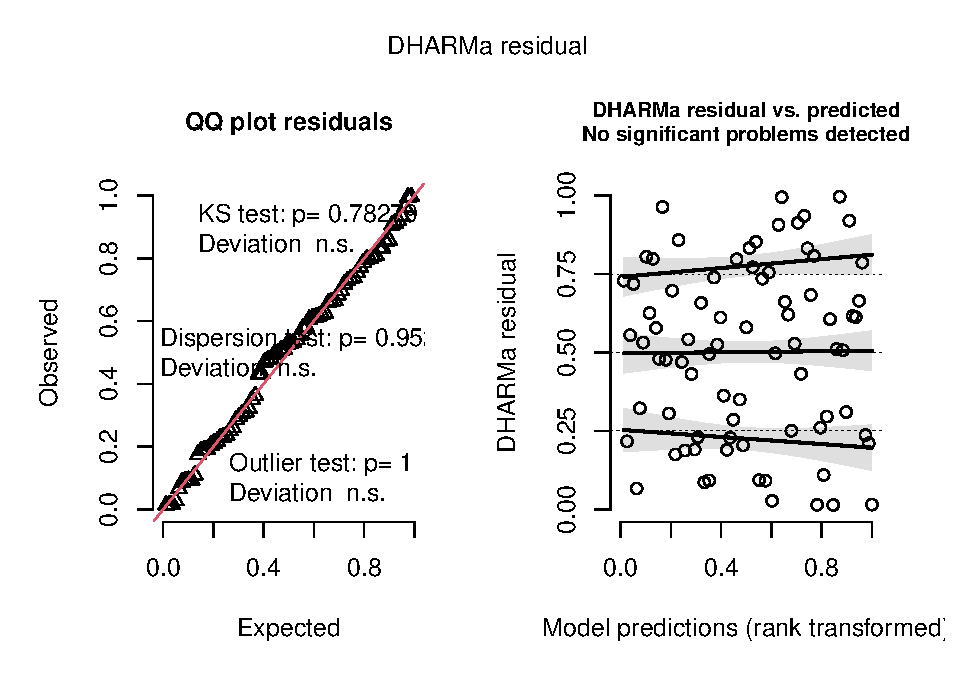
\includegraphics{Supplementary_materials_files/figure-latex/unnamed-chunk-60-2} \end{center}

\subsection{\texorpdfstring{Change in the amount of compounds associated with \emph{F. sanguinea}}{Change in the amount of compounds associated with F. sanguinea}}\label{change-in-the-amount-of-compounds-associated-with-f.-sanguinea}

\begin{verbatim}
## Linear mixed model fit by REML. t-tests use Satterthwaite's method ['lmerModLmerTest']
## Formula: I(sqrt(corrected_mass_part)) ~ poly(mean_delta, 1) + (1 | colony)
##    Data: separation_data[-c(69, 74), ]
## 
## REML criterion at convergence: -87
## 
## Scaled residuals: 
##      Min       1Q   Median       3Q      Max 
## -2.19985 -0.64322  0.04887  0.72139  2.56609 
## 
## Random effects:
##  Groups   Name        Variance Std.Dev.
##  colony   (Intercept) 0.001593 0.03991 
##  Residual             0.016477 0.12836 
## Number of obs: 78, groups:  colony, 11
## 
## Fixed effects:
##                     Estimate Std. Error       df t value Pr(>|t|)    
## (Intercept)          0.53275    0.01916  7.82144   27.81 4.21e-09 ***
## poly(mean_delta, 1)  0.93643    0.12987 69.56931    7.21 5.31e-10 ***
## ---
## Signif. codes:  0 '***' 0.001 '**' 0.01 '*' 0.05 '.' 0.1 ' ' 1
## 
## Correlation of Fixed Effects:
##             (Intr)
## ply(mn_d,1) 0.019
\end{verbatim}

\begin{verbatim}
## 
##  Shapiro-Wilk normality test
## 
## data:  residuals(lm_model)
## W = 0.98446, p-value = 0.4618
\end{verbatim}

\begin{center}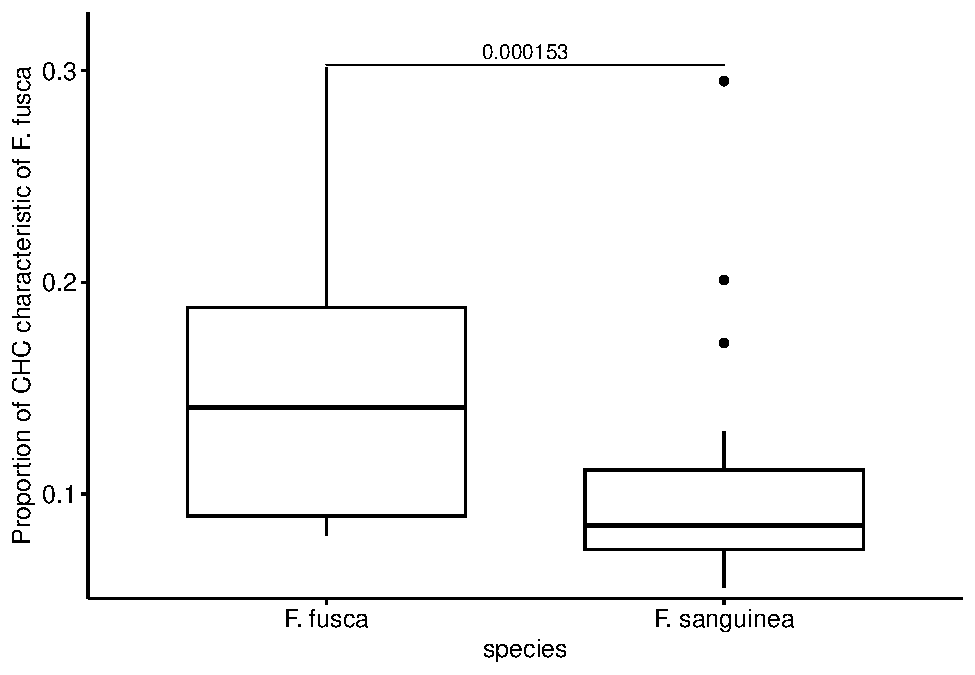
\includegraphics{Supplementary_materials_files/figure-latex/unnamed-chunk-61-1} 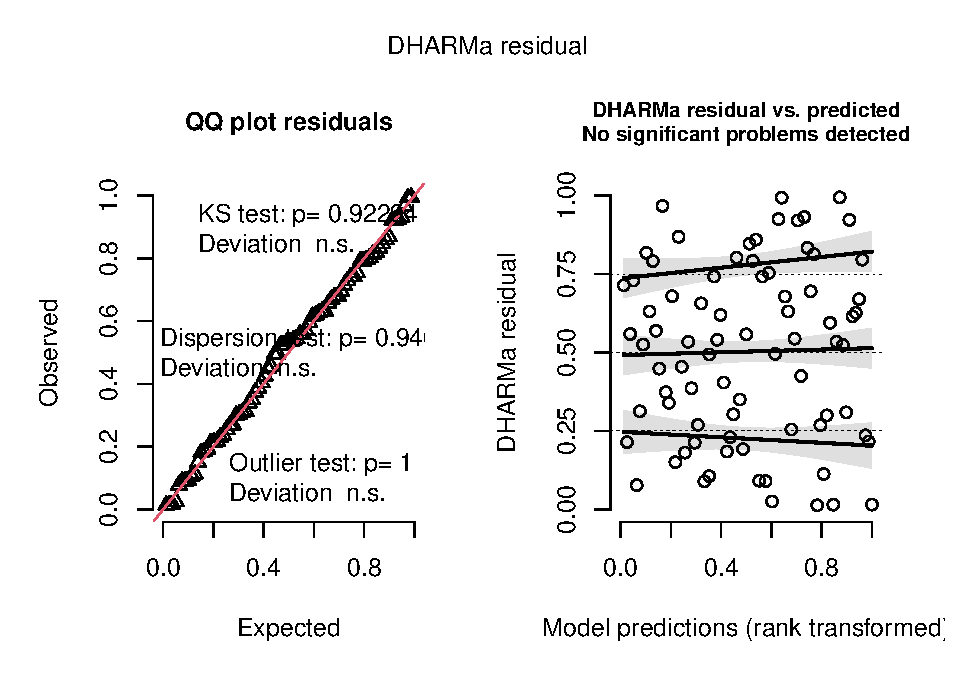
\includegraphics{Supplementary_materials_files/figure-latex/unnamed-chunk-61-2} \end{center}

\subsection{\texorpdfstring{Change in the amount of compounds associated with \emph{F. fusca}}{Change in the amount of compounds associated with F. fusca}}\label{change-in-the-amount-of-compounds-associated-with-f.-fusca}

\begin{verbatim}
## Linear mixed model fit by REML. t-tests use Satterthwaite's method ['lmerModLmerTest']
## Formula: corrected_mass_part ~ mean_delta + (1 | colony)
##    Data: separation_data
## 
## REML criterion at convergence: -171.5
## 
## Scaled residuals: 
##     Min      1Q  Median      3Q     Max 
## -1.8982 -0.6538 -0.1157  0.6326  2.3286 
## 
## Random effects:
##  Groups   Name        Variance Std.Dev.
##  colony   (Intercept) 0.006545 0.08090 
##  Residual             0.003934 0.06272 
## Number of obs: 80, groups:  colony, 11
## 
## Fixed effects:
##               Estimate Std. Error         df t value Pr(>|t|)    
## (Intercept)  0.1739794  0.0267734 11.9815824   6.498 2.97e-05 ***
## mean_delta  -0.0017124  0.0005453 68.3928213  -3.140  0.00249 ** 
## ---
## Signif. codes:  0 '***' 0.001 '**' 0.01 '*' 0.05 '.' 0.1 ' ' 1
## 
## Correlation of Fixed Effects:
##            (Intr)
## mean_delta -0.307
\end{verbatim}

\begin{verbatim}
## 
##  Shapiro-Wilk normality test
## 
## data:  residuals(lm_model)
## W = 0.96856, p-value = 0.04595
\end{verbatim}

\begin{center}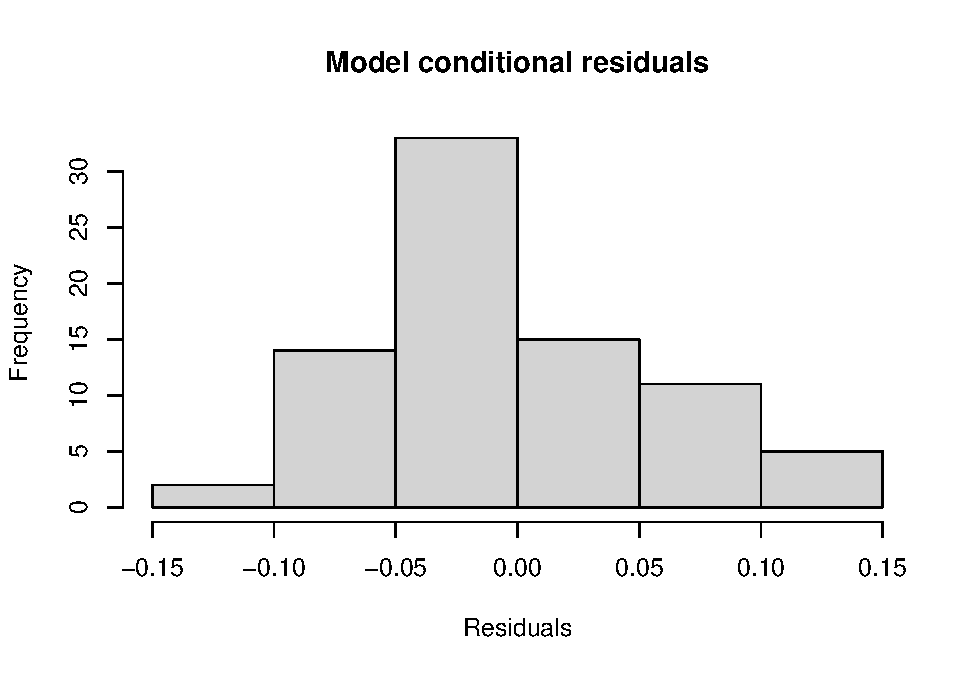
\includegraphics{Supplementary_materials_files/figure-latex/unnamed-chunk-62-1} \includegraphics{Supplementary_materials_files/figure-latex/unnamed-chunk-62-2} \end{center}

\section{\texorpdfstring{Impact of slave on the development of the \emph{F. sanguinea} CHC profile}{Impact of slave on the development of the F. sanguinea CHC profile}}\label{impact-of-slave-on-the-development-of-the-f.-sanguinea-chc-profile}

We analyzed the impact of \emph{F. fusca} slaves on the CHC profile of callow \emph{F. sanguinea} ants. In this experiment, \emph{F. sanguinea} ants were isolated in pairs before eclosion, and their CHC profiles were analyzed at one of four time points marking their adult age. We then tested whether callow \emph{F. sanguinea} ants were chemically more similar to their slave relatives from free-living colonies. Unrelated \emph{F. fusca} ants served as a background group.''

\subsection{Analysis based on all samples}\label{analysis-based-on-all-samples}

\begin{figure}

{\centering \includegraphics[width=0.8\linewidth]{Supplementary_materials_files/figure-latex/unnamed-chunk-64-1} 

}

\caption{Distribution of lifespans of ants used in the experiment. The precise age of individuals could not be determined because ants in pairs were not marked. Therefore, all possible combinations were considered to illustrate the potential range.}\label{fig:unnamed-chunk-64}
\end{figure}

\begin{verbatim}
## Empirical p-value for the chemical distance difference for the ants aged 1-3 days:0.00000
\end{verbatim}

\begin{verbatim}
## Number of colonies used in the treatment of 1-3 days of separation: 9
\end{verbatim}

\begin{verbatim}
## Empirical p-value for the chemical distance difference for the ants aged 8-10 days:0.00000
\end{verbatim}

\begin{verbatim}
## Number of colonies used in the treatment of 8-10 days of separation: 9
\end{verbatim}

\begin{verbatim}
## Empirical p-value for the chemical distance difference for the ants aged 17-20 days:0.00080
\end{verbatim}

\begin{verbatim}
## Number of colonies used in the treatment of 17-20 days of separation: 9
\end{verbatim}

\begin{verbatim}
## Empirical p-value for the chemical distance difference for the ants aged 35-40 days:0.00705
\end{verbatim}

\begin{verbatim}
## Number of colonies used in the treatment of 35-40 days of separation: 8
\end{verbatim}

\begin{table}

\caption{\label{tab:unnamed-chunk-73}Chemical distance of the isolated \textit{F. sanguinea} ant to \textit{F. fusca} ants realted and unrelated to slaves.}
\centering
\begin{tabular}[t]{l|>{\raggedleft\arraybackslash}p{4cm}|>{\raggedleft\arraybackslash}p{4cm}}
\hline
Adult age & Chemical distance to slaves' relatives & Chemical distance to random colonies\\
\hline
1-3 days & 0.3339 & 0.4723\\
\hline
8-10 days & 0.3526 & 0.4809\\
\hline
17-20 days & 0.4533 & 0.5296\\
\hline
35-40 days & 0.5730 & 0.6101\\
\hline
\end{tabular}
\end{table}

\subsection{Analysis restricted to the individuals hatched from cocoons}\label{analysis-restricted-to-the-individuals-hatched-from-cocoons}

Since naked pupae might have acquired CHC through physical contact with adult ants after pupation, we subset our data to include only those samples which derived from the ants hatched from cocoons. In this case silky envelop during pupa stage ruled out possibility of the CHC transfer from the environment.

\begin{verbatim}
## Empirical p-value for the chemical distance difference for the ants aged 1-3 days:0.00000
\end{verbatim}

\begin{verbatim}
## Number of colonies used in the treatment of 1-3 days of separation: 8
\end{verbatim}

\begin{verbatim}
## Empirical p-value for the chemical distance difference for the ants aged 8-10 days:0.00001
\end{verbatim}

\begin{verbatim}
## Number of colonies used in the treatment of 8-10 days of separation: 8
\end{verbatim}

\begin{verbatim}
## Empirical p-value for the chemical distance difference for the ants aged 17-20 days:0.00453
\end{verbatim}

\begin{verbatim}
## Number of colonies used in the treatment of 17-20 days of separation: 8
\end{verbatim}

\begin{verbatim}
## Empirical p-value for the chemical distance difference for the ants aged 35-40 days:0.03298
\end{verbatim}

\begin{verbatim}
## Number of colonies used in the treatment of 35-40 days of separation: 7
\end{verbatim}

\begin{table}

\caption{\label{tab:unnamed-chunk-84}Chemical distance of the isolated \textit{F. sanguinea} ant to \textit{F. fusca} ants realted and unrelated to slaves. Isolated ant spun a silky envelope before pupal stage, which prevented CHC transfer from the enviroment.}
\centering
\begin{tabular}[t]{l|>{\raggedleft\arraybackslash}p{4cm}|>{\raggedleft\arraybackslash}p{4cm}}
\hline
Adult age & Chemical distance to slaves' relatives & Chemical distance to random colonies\\
\hline
1-3 days & 0.3480 & 0.4875\\
\hline
8-10 days & 0.3752 & 0.4941\\
\hline
17-20 days & 0.4655 & 0.5413\\
\hline
35-40 days & 0.6176 & 0.6458\\
\hline
\end{tabular}
\end{table}

\section{Effect of dummy ants}\label{effect-of-dummy-ants}

In these experiments, \emph{F. sanguinea} ants released from their cocoon envelopes were maintained in Petri dishes along with glass beads coated with CHC extracted from either \emph{F. fusca} or \emph{F. sanguinea} ants. We examined whether the contact with dummy nestmates influenced the development of CHC profile of young \emph{F. sanguinea} workers. In particular, we aimed to determine there there is evidence for active chemical mimicry in \emph{F. sanguinea}.

\subsection{\texorpdfstring{Distance to the CHC profile of the dummy ants treated by \emph{F. fusca} CHCs}{Distance to the CHC profile of the dummy ants treated by F. fusca CHCs}}\label{distance-to-the-chc-profile-of-the-dummy-ants-treated-by-f.-fusca-chcs}

We computed the chemical distance to the CHC profile of ants whose CHCs were used to cover glass beads serving as dummy ants. In the control variant, we used the ants subjected to clean glass beads.

\begin{verbatim}
## 
##  Wilcoxon signed rank exact test
## 
## data:  to_test$mean_dist.x and to_test$mean_dist.y
## V = 19, p-value = 0.7344
## alternative hypothesis: true location shift is not equal to 0
\end{verbatim}

\begin{table}

\caption{\label{tab:unnamed-chunk-88}Chemical distance of separated \textit{F. sanguinea} ants to the CHC profile of \textit{F. fusca} ants from colonies that served as a source of CHC to caot the glass beads. In control variant, glass bead were left clean.}
\centering
\begin{tabular}[t]{l|l|>{\raggedleft\arraybackslash}p{2cm}|l|>{\raggedleft\arraybackslash}p{2cm}}
\hline
Colony ID & Treamtent & Averaged distance & Contrast & Averaged distance\\
\hline
SD18-3 & 12-15 days + F. fusca hydrocarbons & 0.3957886 & 12-15 days (control) & 0.5093071\\
\hline
SD18-5 & 12-15 days + F. fusca hydrocarbons & 0.6157811 & 12-15 days (control) & 0.5132649\\
\hline
SD18-5 & 12-15 days + F. fusca hydrocarbons & 0.8423114 & 12-15 days (control) & 0.8316840\\
\hline
SD19-11 & 12-15 days + F. fusca hydrocarbons & 0.4665112 & 12-15 days (control) & 0.4691791\\
\hline
SD19-3 & 12-15 days + F. fusca hydrocarbons & 0.4996918 & 12-15 days (control) & 0.4361776\\
\hline
SD19-4 & 12-15 days + F. fusca hydrocarbons & 0.3049006 & 12-15 days (control) & 0.4244113\\
\hline
SD19-6 & 12-15 days + F. fusca hydrocarbons & 0.6735461 & 12-15 days (control) & 0.6991620\\
\hline
SD19-8 & 12-15 days + F. fusca hydrocarbons & 0.5954873 & 12-15 days (control) & 0.5870741\\
\hline
SD20-2 & 12-15 days + F. fusca hydrocarbons & 0.6985494 & 12-15 days (control) & 0.7087854\\
\hline
\end{tabular}
\end{table}

\subsection{\texorpdfstring{Distance to the CHC profile of the dummy ants treated by \emph{F. sanguinea} CHCs}{Distance to the CHC profile of the dummy ants treated by F. sanguinea CHCs}}\label{distance-to-the-chc-profile-of-the-dummy-ants-treated-by-f.-sanguinea-chcs}

\begin{verbatim}
## 
##  Wilcoxon signed rank exact test
## 
## data:  to_test$mean_dist.x and to_test$mean_dist.y
## V = 15, p-value = 0.2324
## alternative hypothesis: true location shift is not equal to 0
\end{verbatim}

\begin{table}

\caption{\label{tab:unnamed-chunk-89}Chemical distance of separated \textit{F. sanguinea} ants to the CHC profile of \textit{F. sanguinea} ants from colonies that served as a source of CHC to caot the glass beads. In control variant, glass bead were left clean.}
\centering
\begin{tabular}[t]{l|l|>{\raggedleft\arraybackslash}p{2cm}|l|>{\raggedleft\arraybackslash}p{2cm}}
\hline
Colony ID & Treamtent & Averaged distance & Contrast & Averaged distance\\
\hline
SD18-2 & 12-15 days + F. sanguinea hydrocarbons & 0.5706616 & 12-15 days (control) & 0.3734387\\
\hline
SD18-3 & 12-15 days + F. sanguinea hydrocarbons & 0.4565024 & 12-15 days (control) & 0.5986922\\
\hline
SD18-5 & 12-15 days + F. sanguinea hydrocarbons & 0.5246184 & 12-15 days (control) & 0.5800488\\
\hline
SD18-5 & 12-15 days + F. sanguinea hydrocarbons & 0.2501310 & 12-15 days (control) & 0.2323064\\
\hline
SD19-11 & 12-15 days + F. sanguinea hydrocarbons & 0.5953242 & 12-15 days (control) & 0.6070599\\
\hline
SD19-3 & 12-15 days + F. sanguinea hydrocarbons & 0.4185158 & 12-15 days (control) & 0.5112225\\
\hline
SD19-4 & 12-15 days + F. sanguinea hydrocarbons & 0.6477936 & 12-15 days (control) & 0.6680334\\
\hline
SD19-6 & 12-15 days + F. sanguinea hydrocarbons & 0.5525058 & 12-15 days (control) & 0.5908247\\
\hline
SD19-8 & 12-15 days + F. sanguinea hydrocarbons & 0.8501448 & 12-15 days (control) & 0.8499395\\
\hline
SD20-2 & 12-15 days + F. sanguinea hydrocarbons & 0.6460560 & 12-15 days (control) & 0.6543900\\
\hline
\end{tabular}
\end{table}

\subsection{\texorpdfstring{Fraction of \emph{n}-docosane in the CHC profile}{Fraction of n-docosane in the CHC profile}}\label{fraction-of-n-docosane-in-the-chc-profile}

For the control treatment, glass beads were left uncoated with CHC. In the experimental treatments, the CHC used to coat the glass beads were supplemented with \emph{n}-docosane, which served as an internal standard. We examined differences in the proportion of \emph{n}-docosane in the CHC profiles of the tested ants, as these could indicate the acquisition of chemicals from the dummy ants.

\subsubsection{\texorpdfstring{\emph{F. fusca}}{F. fusca}}\label{f.-fusca-2}

\begin{verbatim}
## 
##  Wilcoxon signed rank exact test
## 
## data:  to_test$C22_prop.x and to_test$C22_prop.y
## V = 55, p-value = 0.001953
## alternative hypothesis: true location shift is not equal to 0
\end{verbatim}

\begin{table}

\caption{\label{tab:unnamed-chunk-90}Proportion of \textit{n}-docosane in CHC extracted from \textit{F. sanguinea} ants maintained with the glass beads coated with the CHC of \textit{F. fusca} ants and contaminated with \textit{n}-docosane. In control variant, glass bead were left clean.}
\centering
\begin{tabular}[t]{l|l|>{\raggedleft\arraybackslash}p{2cm}|l|>{\raggedleft\arraybackslash}p{2cm}}
\hline
Colony ID & Treamtent & Averaged C22 fraction & Contrast & Averaged C22 fraction\\
\hline
SD18-3 & 12-15 days + F. fusca hydrocarbons & 0.0178168 & 12-15 days (control) & 0.0000000\\
\hline
SD18-5 & 12-15 days + F. fusca hydrocarbons & 0.0012056 & 12-15 days (control) & 0.0000000\\
\hline
SD18-5 & 12-15 days + F. fusca hydrocarbons & 0.0017152 & 12-15 days (control) & 0.0003274\\
\hline
SD19-11 & 12-15 days + F. fusca hydrocarbons & 0.0112850 & 12-15 days (control) & 0.0019864\\
\hline
SD19-3 & 12-15 days + F. fusca hydrocarbons & 0.0086141 & 12-15 days (control) & 0.0009720\\
\hline
SD19-4 & 12-15 days + F. fusca hydrocarbons & 0.0173323 & 12-15 days (control) & 0.0000000\\
\hline
SD19-6 & 12-15 days + F. fusca hydrocarbons & 0.0091910 & 12-15 days (control) & 0.0011031\\
\hline
SD19-8 & 12-15 days + F. fusca hydrocarbons & 0.0026387 & 12-15 days (control) & 0.0021076\\
\hline
SD20-2 & 12-15 days + F. fusca hydrocarbons & 0.0086688 & 12-15 days (control) & 0.0049489\\
\hline
W17-1 & 12-15 days + F. fusca hydrocarbons & 0.0211912 & 12-15 days (control) & 0.0014942\\
\hline
\end{tabular}
\end{table}

\subsubsection{\texorpdfstring{\emph{F. sanguinea}}{F. sanguinea}}\label{f.-sanguinea}

\begin{verbatim}
## 
##  Wilcoxon signed rank exact test
## 
## data:  to_test$C22_prop.x and to_test$C22_prop.y
## V = 63, p-value = 0.004883
## alternative hypothesis: true location shift is not equal to 0
\end{verbatim}

\begin{longtable}[t]{l|l|>{\raggedleft\arraybackslash}p{2cm}|l|>{\raggedleft\arraybackslash}p{2cm}}
\caption{\label{tab:unnamed-chunk-91}Proportion of *n*-docosane in CHC extracted from \textit{F. sanguinea} ants maintained with the glass beads coated with the CHC of \textit{F. sanguinea} ants and contaminated with \textit{n}-docosane. In control variant, glass bead were left clean.}\\
\hline
Colony ID & Treamtent & Averaged C22 fraction & Contrast & Averaged C22 fraction\\
\hline
SD18-2 & 12-15 days + F. sanguinea hydrocarbons & 0.0050660 & 12-15 days (control) & 0.0016166\\
\hline
SD18-3 & 12-15 days + F. sanguinea hydrocarbons & 0.0141292 & 12-15 days (control) & 0.0000000\\
\hline
SD18-5 & 12-15 days + F. sanguinea hydrocarbons & 0.0032893 & 12-15 days (control) & 0.0000000\\
\hline
SD18-5 & 12-15 days + F. sanguinea hydrocarbons & 0.0021351 & 12-15 days (control) & 0.0003274\\
\hline
SD19-11 & 12-15 days + F. sanguinea hydrocarbons & 0.0040419 & 12-15 days (control) & 0.0019864\\
\hline
SD19-3 & 12-15 days + F. sanguinea hydrocarbons & 0.0032399 & 12-15 days (control) & 0.0009720\\
\hline
SD19-4 & 12-15 days + F. sanguinea hydrocarbons & 0.0017680 & 12-15 days (control) & 0.0000000\\
\hline
SD19-6 & 12-15 days + F. sanguinea hydrocarbons & 0.0035583 & 12-15 days (control) & 0.0011031\\
\hline
SD19-8 & 12-15 days + F. sanguinea hydrocarbons & 0.0017423 & 12-15 days (control) & 0.0021076\\
\hline
SD20-2 & 12-15 days + F. sanguinea hydrocarbons & 0.0043650 & 12-15 days (control) & 0.0049489\\
\hline
W17-1 & 12-15 days + F. sanguinea hydrocarbons & 0.0030204 & 12-15 days (control) & 0.0014942\\
\hline
\end{longtable}

\section{\texorpdfstring{Body surface area of \emph{F. sanguinea} ants and their slaves}{Body surface area of F. sanguinea ants and their slaves}}\label{surface_area}

In the publication, CHC amounts are reported relative to the square of head width. To assess whether this measure reliably reflects body size, we measured the planar projection areas of different body parts of \emph{F. sanguinea} and \emph{F. fusca}. The plots below suggest that head width slightly underestimates body surface area in \emph{F. fusca} compared to \emph{F. sanguinea}. As a result, the relative concentration of CHC in \emph{F. fusca} may be overestimated. However, this bias acts in the opposite direction of our findings---\emph{F. sanguinea} exhibits greater CHC concentration on its cuticle. Therefore, the shape-related bias between species is conservative, as it reduces the likelihood of rejecting the null hypothesis

\begin{figure}

{\centering \includegraphics{Supplementary_materials_files/figure-latex/unnamed-chunk-92-1} 

}

\caption{Ratios of the planar projection areas of three body parts (head, thorax dorsal view, thorax lateral view) to the square of head width.}\label{fig:unnamed-chunk-92}
\end{figure}

  \bibliography{book.bib}

\end{document}
